\documentclass{article}

\usepackage[final]{neurips_2022}
\usepackage[UTF8, fontset=adobe]{ctex}

\usepackage[utf8]{inputenc}
\usepackage[T1]{fontenc}
\usepackage{hyperref}
\usepackage{url}
\usepackage{booktabs}
\usepackage{amsfonts}
\usepackage{nicefrac}
\usepackage{float}
\usepackage{amsmath}
\usepackage{algorithm}
\usepackage{algpseudocode}
\usepackage{microtype}
\usepackage{xcolor}
\usepackage{bm}
\usepackage{graphicx}
\usepackage{subfigure}
\usepackage{listings}

\hypersetup{
    colorlinks=true,
    linkbordercolor=white,
}

\renewcommand{\algorithmicrequire}{\textbf{Input:}}
\renewcommand{\algorithmicensure}{\textbf{Output:}}

\title{大数据分析中的算法期末上机报告}

\author{
    \large 陈润璘 \\
    \large \texttt{2200010848}
    \And
    \large 任子博 \\
    \large \texttt{2200010626}
}

\begin{document}

\maketitle

\section{问题描述}
铁路列车时刻表问题旨在为列车制定一个满足要求的的运行计划,以满足乘客需求并优化资源利用。本次大作业使用多种算法来求解这一问题。

\subsection{时空网络模型}\label{subsec:spatial-temporal-network-model}

铁路列车时刻表问题的时空网络模型旨在通过一个 0-1 整数规划模型来确定一个无冲突的列车运行计划。该模型基于时空网络构建,目标是最大化某种意义上的“利润”。

\subsubsection{目标函数}
模型的目标是最大化所有调度列车在各自路径上所选弧(路段或车站停驻)的“利润”之和:
\begin{equation}
    \max \sum_{j \in J} \sum_{e \in E_j} p_e x_e\label{eq:obj}
\end{equation}
其中,$p_e$ 是使用弧 $e$
的“利润”值。在实现中,“利润”可以有多种实际含义,例如:若将始发弧的利润设为1,其他为0,则目标是最大化运行的列车数量;若将$p_e$设为路段运行时间的相反数,则目标是最小化总运行时间;若将目标函数直接设为0,则仅进行可行性检查。

\subsubsection{决策变量}
\begin{itemize}
    \item $x_e \in \{0,1\}$: 二元决策变量。如果弧 $e \in E$ 被某列车占用,则 $x_e = 1$;否则为 $0$。
    \item $z_{jv}$: 辅助二元变量。如果节点 $v \in V_j$ 被列车 $j \in J$ 占用,则
        $z_{jv} = 1$;否则为 $0$。
    \item $y_v$: 辅助二元变量。如果节点 $v \in V_j$ 被任何列车占用,则 $y_v = 1$;否则为 $0$。
\end{itemize}

\subsubsection{模型参数}
\begin{itemize}
    \item $J$: 所有列车的集合 。
    \item $E_j$: 列车 $j$ 在时空网络中可使用的弧(arc)的集合。
    \item $E$: 时空网络中所有弧的集合, $E = \bigcup_{j \in J} E_j$ 。
    \item $V_j$: 列车 $j$ 在时空网络中可访问的节点(node)的集合 。
    \item $V$: 时空网络中所有节点的集合, $V = \bigcup_{j \in J} V_j$ 。
    \item $p_e$: 列车使用弧 $e$ 所产生的“利润” 。
    \item $\sigma, \tau$: 分别表示时空网络中的虚拟始发节点和虚拟终点节点 。
    \item $\delta_j^+(v)$: 对于列车 $j$,从节点 $v$ 出发的弧的集合 。
    \item $\delta_j^-(v)$: 对于列车 $j$,进入节点 $v$ 的弧的集合 。
    \item $T(v)$: 可能通过节点 $v$ 的所有列车的集合 。
    \item $N(v)$: 与节点 $v$ 相冲突的节点集合(包括 $v$ 本身)。这些节点不能同时被占用 。
\end{itemize}

\subsubsection{约束条件}
\begin{enumerate}
    \item \textbf{列车路径的始发约束}:
        每列车 $j$ 最多只能选择一条从虚拟始发节点 $\sigma$ 出发的弧。这表示每列车最多只能开始其行程一次。
        \begin{equation}
            \sum_{e \in \delta_j^+(\sigma)} x_e \le 1, \quad \forall
            j \in J\label{eq:con_start}
        \end{equation}

    \item \textbf{流量守恒约束}:
        对于每列车 $j$ 和每个非虚拟始发/终点节点
        $v$,进入该节点的被选中的弧的数量必须等于从该节点出发的被选中的弧的数量。这确保了列车路径的连续性。
        \begin{equation}
            \sum_{e \in \delta_j^-(v)} x_e = \sum_{e \in
            \delta_j^+(v)} x_e, \quad \forall j \in J, \forall v \in
            V \setminus \{\sigma, \tau\}\label{eq:con_flow}
        \end{equation}

    \item \textbf{列车路径的终止约束}:
        每列车 $j$ 最多只能选择一条进入虚拟终点节点 $\tau$ 的弧。这表示每列车最多只能结束其行程一次 。
        \begin{equation}
            \sum_{e \in \delta_j^-(\tau)} x_e \le 1, \quad \forall j
            \in J\label{eq:con_end}
        \end{equation}

    \item \textbf{节点占用逻辑约束}:
        定义了节点 $v$ 是否被列车 $j$ 占用 ($z_{jv}$)。如果列车 $j$ 使用了任何一条进入节点 $v$
        的弧,则该节点被列车 $j$ 占用。
        \begin{equation}
            z_{jv} = \sum_{e \in \delta_j^-(v)} x_e, \quad \forall j
            \in J, \forall v \in V_j\label{eq:con_node_occupied}
        \end{equation}

    \item \textbf{节点总体占用逻辑约束}:
        定义了节点 $v$ 是否被任何列车占用 ($y_v$)。如果至少有一列车占用了节点 $v$,则 $y_v=1$。
        \begin{equation}
            y_v = \sum_{j \in T(v)} z_{jv}, \quad \forall v \in
            V_j\label{eq:con_node_occupied_total}
        \end{equation}

    \item \textbf{Headway (最小间隔) 约束}:
        对于网络中的任何节点 $v$,其冲突集合 $N(v)$
        中的所有节点(这些节点代表了在时间或空间上不能同时占用的状态),最多只能有一个被占用。这是为了避免列车冲突,保证运行安全。
        \begin{equation}
            \sum_{v' \in N(v)} y_{v'} \le 1, \quad \forall v \in
            V\label{eq:con_headway}
        \end{equation}

    \item \textbf{二元变量约束}:
        所有决策变量 $x_e$ 都必须是0或1。
        \begin{equation}
            x_e \in \{0,1\}, \quad \forall e \in E\label{eq:con_binary}
        \end{equation}
\end{enumerate}

\subsection{Job-Shop调度模型}\label{subsec:job-shop}

\subsubsection{目标函数}
Job-Shop 调度模型支持三种目标函数:

\begin{enumerate}
    \item \textbf{最小化所有列车到达终点站的总时间}:
        \begin{equation}
            \min \sum_{j \in J} a_{j, S}\label{eq:min_sum_arrival}
        \end{equation}
        其中 $a_{j, S}$ 表示列车 $j$ 到达终点站 $S$ 的时间。

    \item \textbf{最小化最大完工时间}:
        \begin{equation}
            \min C_{\max} , \ \ \text{where} \ C_{\max} = \max_{j \in J}
            a_{j, S}\label{eq:min}
        \end{equation}

    \item \textbf{可行性检查}:
        \begin{equation}
            \min 0\label{eq:feasibility}
        \end{equation}
        仅判断约束是否可行,不优化具体目标。
\end{enumerate}

\subsubsection{决策变量}
\begin{itemize}
    \item $a_{j,s}$: 连续变量,表示列车 $j \in J$ 到达车站 $s \in \{1, \dots, N_S-1\}$ 的时间。
    \item $d_{j,s}$: 连续变量,表示列车 $j \in J$ 从车站 $s \in \{0, \dots, N_S-2\}$ 出发的时间。
    \item $\delta^{arr}_{j_1,j_2,s}$: 二元变量,用于处理列车 $j_1, j_2 \in J$
        ($j_1 \neq j_2$) 在车站 $s \in \{1, \dots, N_S-1\}$ 的到达间隔。如果
        $j_1$ 在 $j_2$ 之前(或同时)到达,则可能为1,否则为0(具体取决于约束的精确形式)。
    \item $\delta^{dep}_{j_1,j_2,s}$: 二元变量,用于处理列车 $j_1, j_2 \in J$
        ($j_1 \neq j_2$) 在车站 $s \in \{0, \dots, N_S-2\}$ 的出发间隔。如果
        $j_1$ 在 $j_2$ 之前(或同时)出发,则可能为1,否则为0。
    \item $\pi_{j_1,j_2,s}$: 二元变量,表示列车 $j_1, j_2 \in J$ ($j_1 \neq
        j_2$) 在始发站为 $s \in \{0, \dots, N_S-2\}$ 的运行区段 $(s, s+1)$
        上的运行顺序。如果 $j_1$ 先于(或同时于) $j_2$ 通过该区段,则为1,否则为0。
    \item $C_{max}$: 连续变量,表示所有列车的最大完工时间(即最晚到达终点站的时间)。仅在目标函数为
        \texttt{min\_makespan} 时使用。
\end{itemize}

\subsubsection{模型参数}
\begin{itemize}
    \item $J$: 所有列车的集合。
    \item $N_S$: 车站的总数量。车站索引从 $0$ (始发站) 到 $N_S-1$ (终点站)。
    \item $R_{j,s,s+1}$: 列车 $j$ 在区段 $(s, s+1)$ 的纯运行时间。
    \item $D_{min\_stop}$: 列车在停靠站的最小停站时间。
    \item $D_{max\_stop}$: 列车在停靠站的最大停站时间。
    \item $D_{pass}$: 列车通过不停站时的名义停站时间(通常为0)。
    \item $H$: 最小安全行车间隔时间 (Headway)。
    \item $T_{max}$: 列车运行图的最大允许时间范围。
    \item $M$: 一个足够大的正数,用于线性化逻辑约束。
    \item $\epsilon$: 一个很小的正数,用于在约束中严格不等关系。
    \item $is\_stop_{j,s}$: 一个指示参数,如果列车 $j$ 计划在车站 $s$ 停站,则为真(或1),否则为假(或0)。
\end{itemize}

\subsubsection{约束条件}
\begin{enumerate}
    \item \textbf{运行时间约束 (Travel Time Constraints)}: 对于每列车 $j \in J$
        和每个运行区段 $(s, s+1)$ (其中 $s \in \{0, \dots, N_S-2\}$):
        \begin{equation}
            a_{j,s+1} = d_{j,s} + R_{j,s,s+1}\label{eq:travel_time}
        \end{equation}

    \item \textbf{停站时间约束 (Dwell Time Constraints)}: 对于每列车 $j \in J$
        和每个中间车站 $s \in \{1, \dots, N_S-2\}$:
        \begin{itemize}
            \item 如果列车 $j$ 在车站 $s$ 停站 ($is\_stop_{j,s} = \text{true}$):
                \begin{equation}
                    \begin{aligned}
                        d_{j,s} &\ge a_{j,s} + D_{min\_stop} \\
                        d_{j,s} &\le a_{j,s} + D_{max\_stop}
                    \end{aligned}\label{eq:dwell_time}
                \end{equation}
            \item 如果列车 $j$ 在车站 $s$ 通过 ($is\_stop_{j,s} = \text{false}$):
                \begin{equation}
                    d_{j,s} = a_{j,s} + D_{pass}\label{eq:dwell_time2}
                \end{equation}
        \end{itemize}

    \item \textbf{到达间隔约束 (Arrival Headway Constraints)}: 对于任意两列不同的列车
        $j_1, j_2 \in J$ ($j_1 \neq j_2$) 和每个车站 $s \in \{1, \dots,
        N_S-1\}$ (非始发站):
        \begin{equation}
            \begin{aligned}
                a_{j_2,s} &\ge a_{j_1,s} + H - M \cdot (1 -
                \delta^{arr}_{j_1,j_2,s}) \\
                a_{j_1,s} &\ge a_{j_2,s} + H - M \cdot \delta^{arr}_{j_1,j_2,s}
            \end{aligned}\label{eq:arrival_headway}
        \end{equation}

    \item \textbf{出发间隔约束 (Departure Headway Constraints)}:
        对于任意两列不同的列车 $j_1, j_2 \in J$ ($j_1 \neq j_2$) 和每个车站 $s \in
        \{0, \dots, N_S-2\}$ (非终点站):
        \begin{equation}
            \begin{aligned}
                d_{j_2,s} &\ge d_{j_1,s} + H - M \cdot (1 -
                \delta^{dep}_{j_1,j_2,s}) \\
                d_{j_1,s} &\ge d_{j_2,s} + H - M \cdot \delta^{dep}_{j_1,j_2,s}
            \end{aligned}
            \label{eq:departure_headway}
        \end{equation}

    \item \textbf{区间占用顺序约束 (Block Section Order - FIFO)}: 对于任意两列不同的列车
        $j_1, j_2 \in J$ ($j_1 \neq j_2$) 和每个运行区段的始发车站 $s \in \{0,
        \dots, N_S-2\}$ (该区段为 $s \to s+1$):
        \begin{equation}
            \begin{aligned}
                d_{j_1,s} &\le d_{j_2,s} + M \cdot (1 - \pi_{j_1,j_2,s}) \\
                a_{j_1,s+1} &\le a_{j_2,s+1} + M \cdot (1 - \pi_{j_1,j_2,s}) \\
                d_{j_2,s} &\le d_{j_1,s} - \epsilon + M \cdot \pi_{j_1,j_2,s} \\
                a_{j_2,s+1} &\le a_{j_1,s+1} + M \cdot \pi_{j_1,j_2,s}
            \end{aligned}
            \label{eq:block_section_order}
        \end{equation}
        这些约束确保如果 $\pi_{j_1,j_2,s}=1$,则列车 $j_1$ 在区段 $(s, s+1)$ 上先于或同时于
        $j_2$ 出发和到达;如果 $\pi_{j_1,j_2,s}=0$,则 $j_2$ 严格先于 $j_1$ 从车站 $s$
        出发,并先于或同时于 $j_1$ 到达车站 $s+1$。

    \item \textbf{时间窗约束 (Time Window Constraints)}: 对于每列车 $j \in J$:
        \begin{itemize}
            \item 列车到达终点站 $N_S-1$ 的时间不晚于 $T_{max}$:
                \begin{equation}
                    a_{j,N_S-1} \le T_{max}\label{eq:arrival_time_max}
                \end{equation}
            \item 列车从所有非终点站 $s \in \{0, \dots, N_S-2\}$ 出发的时间不晚于 $T_{max}$:
                \begin{equation}
                    d_{j,s} \le T_{max}\label{eq:departure_time_max}
                \end{equation}
        \end{itemize}

    \item \textbf{变量定义域约束 (Variable Domain Constraints)}:
        \begin{itemize}
            \item 所有到达和出发时间为非负连续变量: $a_{j,s} \ge 0$, $d_{j,s} \ge 0$。
            \item 所有 $\delta^{arr}_{j_1,j_2,s}$,
                $\delta^{dep}_{j_1,j_2,s}$, $\pi_{j_1,j_2,s}$
                变量为二元变量, 即 $\in \{0,1\}$。
            \item 如果使用 $C_{max}$,则 $C_{max} \ge 0$。
        \end{itemize}

    \item \textbf{Makespan 约束} (仅当目标为最小化最大完工时间时): 对于每列车 $j \in J$:
        \begin{equation}
            C_{max} \ge a_{j,N_S-1}\label{eq:makespan_constraint}
        \end{equation}
\end{enumerate}

\section{算法描述}
\label{sec:algo_desc}

\subsection{拉格朗日松弛算法 (Lagrangian Relaxation
Solver)}\label{subsec:-(lagrangian-relaxation-solver)}
拉格朗日松弛算法是一种用于求解整数规划问题的近似方法,特别适用于具有复杂约束的调度问题。该方法通过将某些约束引入目标函数中,并使用拉格朗日乘子来调整这些约束的影响,从而简化问题求解。
本次作业基于拉格朗日松弛框架,主要针对时空网络模型中的 headway 约束(式 \ref{eq:con_headway})
进行松弛,算法伪代码如 \ref{alg:lagrangian_relaxation} 所示。

\begin{algorithm}[h]
    \caption{Lagrangian Relaxation Solver}
    \begin{algorithmic}[1]
        \Require 问题数据 (时空网络, 列车信息, headway 定义)
        \Ensure 近似最优且可行的列车路径集合 $X^*$
        \State 初始化拉格朗日乘子 $\lambda_q \ge 0$ (针对 headway 约束 $q$)
        \State 初始化步长 $\eta > 0$, 上下界 $LB, UB$, 最优可行解 $X^*$
        \For{$k = 1 \dots K_{max}$ (最大迭代次数)}
        \ForAll{列车 $j \in J$}
        \State 根据当前 $\lambda$ 计算修正后的弧利润 $p'_e = p_e -
        \text{penalty}(\lambda, e)$
        \State 求解列车 $j$ 的最长路径问题得到路径 $X^k_j$ 及其对偶利润
        \EndFor
        \State 计算当前拉格朗日对偶函数值 $L_k(\lambda) = $ 所有列车对偶利润之和 + $\sum \lambda_q$
        \State 更新上界 $UB = \min(UB, L_k(\lambda))$
        \State 使用启发式方法得到可行路径集 $X_{feas}$
        和目标值 $Z_{feas}$
        \If{$Z_{feas} > LB$}
        \State 更新下界 $LB = Z_{feas}$
        \State $X^* = X_{feas}$
        \EndIf
        \If{满足终止条件}
        \State \textbf{break}
        \EndIf
        \State 计算 headway 约束的违反度 $g_q$
        \State $\lambda_q \gets \max(0, \lambda_q + \eta \cdot g_q)$
        \State 更新步长 $\eta$
        \EndFor
        \State \Return 最优可行解 $X^*$
    \end{algorithmic}\label{alg:lagrangian_relaxation}
\end{algorithm}

\textbf{构造松弛问题}:
Headway 约束 $\sum_{v' \in N(v)} y_{v'} \le 1$
被引入目标函数中,带有拉格朗日乘子 $\lambda_q$。松弛后的目标函数变为 $\max
\sum_{j \in J} \sum_{e \in E_j} p_e x_e - \sum_q \lambda_q
(\sum_{v' \in N(q)} y_{v'} - 1)$。

\textbf{子问题求解}:
对于每个列车 $j$,原问题可以视作为一个最长路径问题(利润最大化)并使用动态规划求解。 弧的利润根据原始利润 $p_e$ 和由
$\lambda_q$导出的惩罚项进行调整。即如果选择的弧 $e=(u,v)$ 的终点节点 $v_n$ (若为物理节点)
位于一个或多个 headway 窗口内,其利润会减去相应的 $\sum \lambda_q$。

\textbf{拉格朗日乘子更新}:
乘子 $\lambda_q$ 根据次梯度法进行更新: $\lambda_q^{k+1} =
\max(0, \lambda_q^k + \eta \cdot (\sum_{v' \in N(q)}
y_{v'}^{k} - 1))$,其中 $\eta$ 是步长,$\sum
y_{v'}^{k}$ 是在第 $k$ 次迭代的子问题解中,所有列车共同导致 headway 约束 $q$
的冲突节点总占用数。

\textbf{启发式方法构造可行解}:
由于拉格朗日松弛的解可能不满足被松弛的 headway
约束,因此采用启发式方法构造可行解。将列车按其在对偶子问题中的目标值(包含乘子惩罚的路径利润)进行降序排序,
依次为每列车寻找一条路径,该路径不与已调度列车的路径发生 headway
冲突。此步骤也通过求解(不含惩罚项的原始利润的)最长路径问题完成,但在构建图时会移除与已选路径冲突的弧(即,如果一个节点
$v'$ 因选择后会导致与已占用节点冲突,则不考虑指向 $v'$ 的弧)。

\textbf{界更新与停机判断}:
拉格朗日对偶问题的解提供了原始问题最优解的一个上界 (UB) ,启发式方法得到的最好可行解的目标值提供了下界 (LB)。
故算法在达到最大迭代次数或UB-LB 间隙足够小或 $\eta$ 过小时终止。

\subsection{交替方向乘子法 (ADMM)}\label{subsec:-(admm)}
交替方向乘子法 (ADMM)
是一种用于求解分布式优化问题的迭代算法,此算法将原始问题分解为更易处理的子问题,并通过对偶变量协调这些子问题的解。本次作业实现了 ADMM
算法在时空网络模型中的应用,针对列车路径选择和 headway 约束进行优化,算法伪代码如 \ref{alg:algorithm} 所示。

\begin{algorithm}[h]
    \caption{ADMM算法主要流程}
    \begin{algorithmic}[1]
        \Require 问题数据 (时空网络, 列车信息, headway 定义)
        \Ensure 近似最优且可行的列车路径集合 $X_{best}^*$
        \State 初始化局部占用 $z_{local_{jv}}$, 全局占用 $z_{global_{jv}}$, 对偶变量 $\mu_{jv}$
        \State 初始化惩罚参数 $\rho > 0$
        \State $X_{best}^* \gets \emptyset$,
        $\text{best\_feasibility} \gets \infty$,
        $\text{best\_objective} \gets -\infty$
        \For{$k = 1 \dots K_{max}$ (最大迭代次数)}
        \State \Comment{1. x-update (更新列车路径 $X^{k+1}$ 和局部占用 $z_{local}^{k+1}$)}
        \ForAll{列车 $j \in J$}
        \State 根据 $p_e, \mu^k, z_{global}^k, \rho$ 计算修正的弧利润
        \State 求解列车 $j$ 的最长路径问题,得到 $X_j^{k+1}$ 和对应的 $z_{local,j}^{k+1}$
        \EndFor
        \State 合并得到 $X^{k+1}$ 和 $z_{local}^{k+1}$
        \State \Comment{2. z-update (更新全局占用 $z_{global}^{k+1}$)}
        \State 对于每个 (车站, 类型) 对:
        \State \quad 根据 $\mu^k, z_{local}^{k+1}, \rho$ 计算节点占用成本
        \State \quad 使用动态规划求解,选择一组满足 headway 约束的 $(v_t, j^*_{v_t})$
        来确定 $z_{global}^{k+1}$
        \State \Comment{3. $\mu$-update (更新对偶变量 $\mu^{k+1}$)}
        \State $\mu_{jv}^{k+1} \gets \mu_{jv}^k + \rho
        (z_{local,jv}^{k+1} - z_{global,jv}^{k+1})$
        \State 更新惩罚参数 $\rho$
        \State 评估当前解 $X^{k+1}$ 的目标值和可行性
        \If{当前解优于 $X_{best}^*$}
        \State 更新 $X_{best}^*$, $\text{best\_feasibility}$,
        $\text{best\_objective}$
        \EndIf
        \If{满足终止条件}
        \State \textbf{break}
        \EndIf
        \EndFor
        \State \Return $X_{best}^*$
    \end{algorithmic}\label{alg:algorithm}
\end{algorithm}

\textbf{问题重述}:
为将时空网络模型中的列车路径选择和 headway 约束转化为 ADMM,我们引入辅助全局变量
$z_{global_{jv}}$,表示列车 $j$ 是否占用节点 $v$。求解目标转化为最大化 $\sum p_e x_e$。
转化后,主要约束是 $z_{local_{jv}} = z_{global_{jv}}$。其中,$z_{local_{jv}}$ 是由
$x_e$ 导出的局部占用变量 (即如果列车 $j$ 的路径包含$v$,则 $z_{local_{jv}}=1$)。

\textbf{ADMM 迭代步骤}:
\begin{enumerate}
    \item \textbf{x-update}:
        对于给定的 $z_{global}$ 和对偶变量 $\mu$ (对应
        $z_{local} - z_{global} = 0$ 的拉格朗日乘子),求解关于
        $x_e$ (以及隐式的 $z_{local}$) 的子问题。
        目标函数为 $\min \sum p_e x_e + \sum_{j,v} \mu_{jv}
        (z_{local_{jv}} - z_{global_{jv}}) +
        \frac{\rho}{2} \sum_{j,v} ||z_{local_{jv}} -
        z_{global_{jv}}||_2^2$。在实现中,针对每个列车
        $j$,使用动态规划求解此最长路径问题。
    \item \textbf{z-update}:
        对于给定的 $z_{local}$ 和 $\mu$,求解关于 $z_{global}$ 的子问题。
        目标函数为 $\min \sum_{j,v} [-\mu_{jv}
            z_{global_{jv}} + \frac{\rho}{2}
        (z_{local_{jv}} - z_{global_{jv}})^2]$,要求满足
        headway 约束 $\sum_{j} z_{global_{jv'}} \le 1$
        对于任意冲突集合 $N(v)$ 中的 $v'$。具体实现中,可以对此子问题进一步分解:对于每个 (station, type)
        对,均通过动态规划解决。首先计算每个 $(j,v)$ 对的成本 $d_{jv} =-\mu_{jv} +
        \frac{\rho}{2} (1 - 2
        z_{local_{jv}})$。然后对每个 $(s, type)$,找到一组时间点$\{t_k\}$ 和对应的列车
        $\{j_k^*\}$,使得
        $z_{global_{j_k^*, (s,type,t_k)}}=1$ 且满足 headway,同时最小化 $\sum
        d_{j_k^*, (s,type,t_k)}$。
    \item \textbf{$\mu$-update}:
        更新对偶变量:$\mu_{jv}^{k+1} = \mu_{jv}^k + \rho
        (z_{local_{jv}}^k - z_{global_{jv}}^k)$。其中惩罚参数 $\rho$ 可在迭代过程中动态调整
\end{enumerate}

\textbf{停机标准与可行性}:
算法迭代直至原始残差 ($||z_{local} - z_{global}||_2$) 足够小且解可行,或达到最大迭代次数。
最终解的可行性通过检查 $z_{global}$ 是否满足所有列车的路径约束和 headway 约束来验证。

\subsection{强化学习}

强化学习(RL)是一种通过与环境交互来学习最优策略的机器学习方法。本次作业中,我们将列车调度问题建模为一个强化学习任务,使用深度强化学习方法来寻找最优的列车运行路径和时刻表。

\subsubsection{马尔可夫决策过程(MDP)建模}
我们将该问题建模为一个马尔可夫决策过程(MDP),定义状态、动作、转移和奖励函数。根据优先级顺序调度的方式,我们将按照一定的优先级顺序依次安排列车的运行路径。对于每列列车,决定其完整的路径,包括各车站的出发和到达时间。

\textbf{状态空间 ($S$):}
在第 $t$ 步决策时的状态 $s_t$ 由当前部分时刻表、当前待安排列车、未安排的列车列表和轨道占用信息组成。
\begin{itemize}
    \item 当前部分时刻表:包含已安排列车(1 到 $t-1$ 列车)的运行路径(各车站的到达与出发时间)。
    \item 当前待安排列车(第 $t$ 列车)的特征:包括其路线(经过的车站序列)、速度、以及必须停靠的站点。
    \item 未安排的列车列表:包含所有尚未安排的列车($t+1$ 到 $N$ 列车)。
    \item 轨道占用信息:从部分时刻表中得出,显示轨道段和车站站台的占用情况。
\end{itemize}

\textbf{动作空间 ($A$):}
对于当前正在安排的列车 $t$,动作 $a_t$ 包括:
\begin{itemize}
    \item 当前列车从起点站的出发时间。
    \item 每个允许或必须停靠的车站上的停留时间。停留时间必须在最小和最大允许范围内。
\end{itemize}

\textbf{转移函数($P(s_{t+1} | s_t, a_t)$):}
给定当前状态 $s_t$ 和动作 $a_t$,下一状态 $s_{t+1}$ 是确定性的。新状态由将列车 $t$
的新安排路径加入到部分时刻表中形成。随后焦点转移到优先级列表中的下一列车 $t+1$。如果所有列车都已安排完毕,则进入终止状态。

\textbf{奖励函数($R(s_t, a_t, s_{t+1})$):}
奖励函数引导智能体寻找可行且高效的时刻表。
\begin{itemize}
    \item 如果某个动作导致不可调和的间隔冲突,则给予较大的负奖励。
    \item 对较长的总运行时间或过长的停留时间给予较小的惩罚,以鼓励效率提升。
    \item 成功安排完一部分或全部列车后给予正向奖励。
\end{itemize}

\subsubsection{处理间隔时间约束}
间隔时间约束对于避免冲突和确保运行可行性至关重要。我们使用屏蔽无效动作的方法来防止违反这些约束。在智能体选择动作(列车的出发和停留时间)之前,系统会识别并禁止可能导致与已有列车冲突的动作。如果某一列车的所有可能动作都不可避免地导致冲突,则可在奖励函数中引入较大惩罚,并终止该轮训练,表示无法生成完整无冲突的时刻表。

\subsubsection{问题特征}
策略网络在决定列车 $t$ 的运行计划时的输入特征可以分为静态特征和动态特征,具体包括:
\begin{itemize}
    \item \textbf{静态特征:}
        \begin{itemize}
            \item 列车 $t$ 的特性:速度、强制停靠站、允许的停留时间范围。
            \item 车站数据:各车站之间的距离。
            \item 列车 $t$ 速度下的区段运行时间。
        \end{itemize}
    \item \textbf{动态特征:}
        \begin{itemize}
            \item 当前时间。
            \item 各轨道段和车站站台的可用窗口,考虑已安排列车 1 到 $t-1$ 的时刻表。
            \item 列车 $t$ 从起点站最早可出发时间,及其后续各站的最早/最晚出发与到达时间。
            \item 为维持连接关系或整体时刻表长度所需的最晚到达时间。
        \end{itemize}
\end{itemize}

\subsubsection{策略网络结构}
可以采用深度神经网络,例如图神经网络(GNN)或循环神经网络(如 LSTM)。在 GNN 中,铁路网络(车站和轨道)可以用图表示。
GNN 可以捕捉车站和轨道段之间的空间关系和依赖性。在 RNN/LSTM 中,将已经安排的列车时刻表作为隐藏状态输入,动态更新状态以捕捉时间序列特性。

\subsubsection{RL 训练流程}
适合使用的策略梯度算法如 \textbf{REINFORCE} 或 \textbf{近端策略优化(PPO)}。
REINFORCE 是一种蒙特卡洛策略梯度方法,基于整个回合的回报更新策略参数。实现较简单但方差较高,可能出现训练不稳定或收敛慢的情况。
PPO 采用的 actor-critic 算法,通过限制策略更新来提供更稳定的训练性能,通常比 REINFORCE
表现更好。训练过程如算法 \ref{alg:train_schedule} 所示。

\begin{algorithm}[h]
    \caption{基于强化学习的列车调度策略训练流程}
    \label{alg:train_schedule}
    \begin{algorithmic}[1]
        \State 初始化策略网络参数 $\theta$
        \Repeat
        \State 重置环境状态
        \State 定义列车调度的优先级顺序
        \For{每一列待调度列车}
        \State 观察当前环境状态 $s_t$
        \State 计算有效动作集合,屏蔽违反间隔时间限制的动作
        \State 根据策略网络 $\pi_\theta$ 采样一个动作 $a_t$
        \State 执行动作 $a_t$,更新全局时刻表并获得奖励 $r_t$
        \State 存储转移 $(s_t, a_t, r_t, s_{t+1})$
        \EndFor
        \State 计算该回合的折扣回报
        \State 使用PPO等算法更新策略网络参数 $\theta$
        \Until{策略收敛或达到期望性能}
    \end{algorithmic}
\end{algorithm}

\section{评价指标}
在本次实验中,我们采用以下指标来评价算法的性能:
\begin{itemize}
    \item \textbf{CPU Time}:算法的运行时间。
    \item \textbf{Iter}:算法停机时的迭代次数。
    \item \textbf{Infeasibility}:算法停机时的约束违反度,即违反的约束数量,$0$表示算法找到原问题可行解。
    \item \textbf{Variables}:算法使用的决策变量的数目。
    \item \textbf{Constraints}:算法使用的约束的数目。
\end{itemize}

\section{实验方法及结果}
本次实验中,使用 Gurobi
求解器对时空网络模型 (\ref{subsec:spatial-temporal-network-model}) 和 Jobshop
(\ref{subsec:job-shop})
模型进行求解,优化目标分别为\texttt{feasibility}、\texttt{min\_makespan}和\texttt{min\_arrive}。
同时,还实现了基于 Lagrangian
Relaxation (\ref{subsec:-(lagrangian-relaxation-solver)}) 和 ADMM
(\ref{subsec:-(admm)}) 的求解算法,各算法求解结果如表 \ref{tab:results} 所示。

\begin{table}[htbp]
    \centering
    \caption{所有算法的性能指标对比\protect\footnotemark[1]}
    \label{tab:results}
    \resizebox{\textwidth}{!}{
        \begin{tabular}{lcccccc}
            \toprule
            Solver             & Obj           & CPU Time(s) & Iter
            & Infeasibility & Variables & Constraints \\ \midrule
            gurobi\_solver     & feasibility   & 129.95      & -
            & 0             & 197678    & 71299       \\
            gurobi\_solver     & min\_makespan & 621.57      & -
            & 0             & 197679    & 73875       \\
            gurobi\_solver     & min\_arrive   & 238.65      & -
            & 0             & 197678    & 71299       \\
            gurobi\_solver(LR) & feasibility   & 4.49        & 250
            & -             & 197678    & 71299       \\
            gurobi\_solver(LR) & min\_makespan & 3.61        & 4441
            & -             & 197679    & 73875       \\
            gurobi\_solver(LR) & min\_arrive   & 1.73        & 4769
            & -             & 197678    & 71299       \\
            job\_shop\_solver  & feasibility   & 1.40        & 60021
            & 0             & 2352      & 6111        \\
            admm\_slover       & feasibility   & 270.39      & 1716
            & 0             & -         & -           \\
            lagrange\_slover   & max\_train    & 716.83      &
            1000(max) & 4 train       & -         & -           \\
            \bottomrule
        \end{tabular}
    }
\end{table}

\footnotetext[1]{Lagrangian Relaxation 算法目标设为在规定时间内安排尽量多的火车,最终有4辆车无法排下。
Gurobi 求解器的在求解时空网络模型是使用的不是简单的迭代法,故无法统计迭代次数。}

各算法得到的铁路时刻图如图 \ref{fig:time_graph_1} 和 \ref{fig:time_graph_2}
所示,其中,直接使用Gurobi求解拉格朗日松弛问题并不能得到可行的排期,故不予展示。

\begin{figure}[htbp]
    \centering
    % 第一页放前 3 张图
    \subfigure[gurobi\_solver\_feasibility]{
        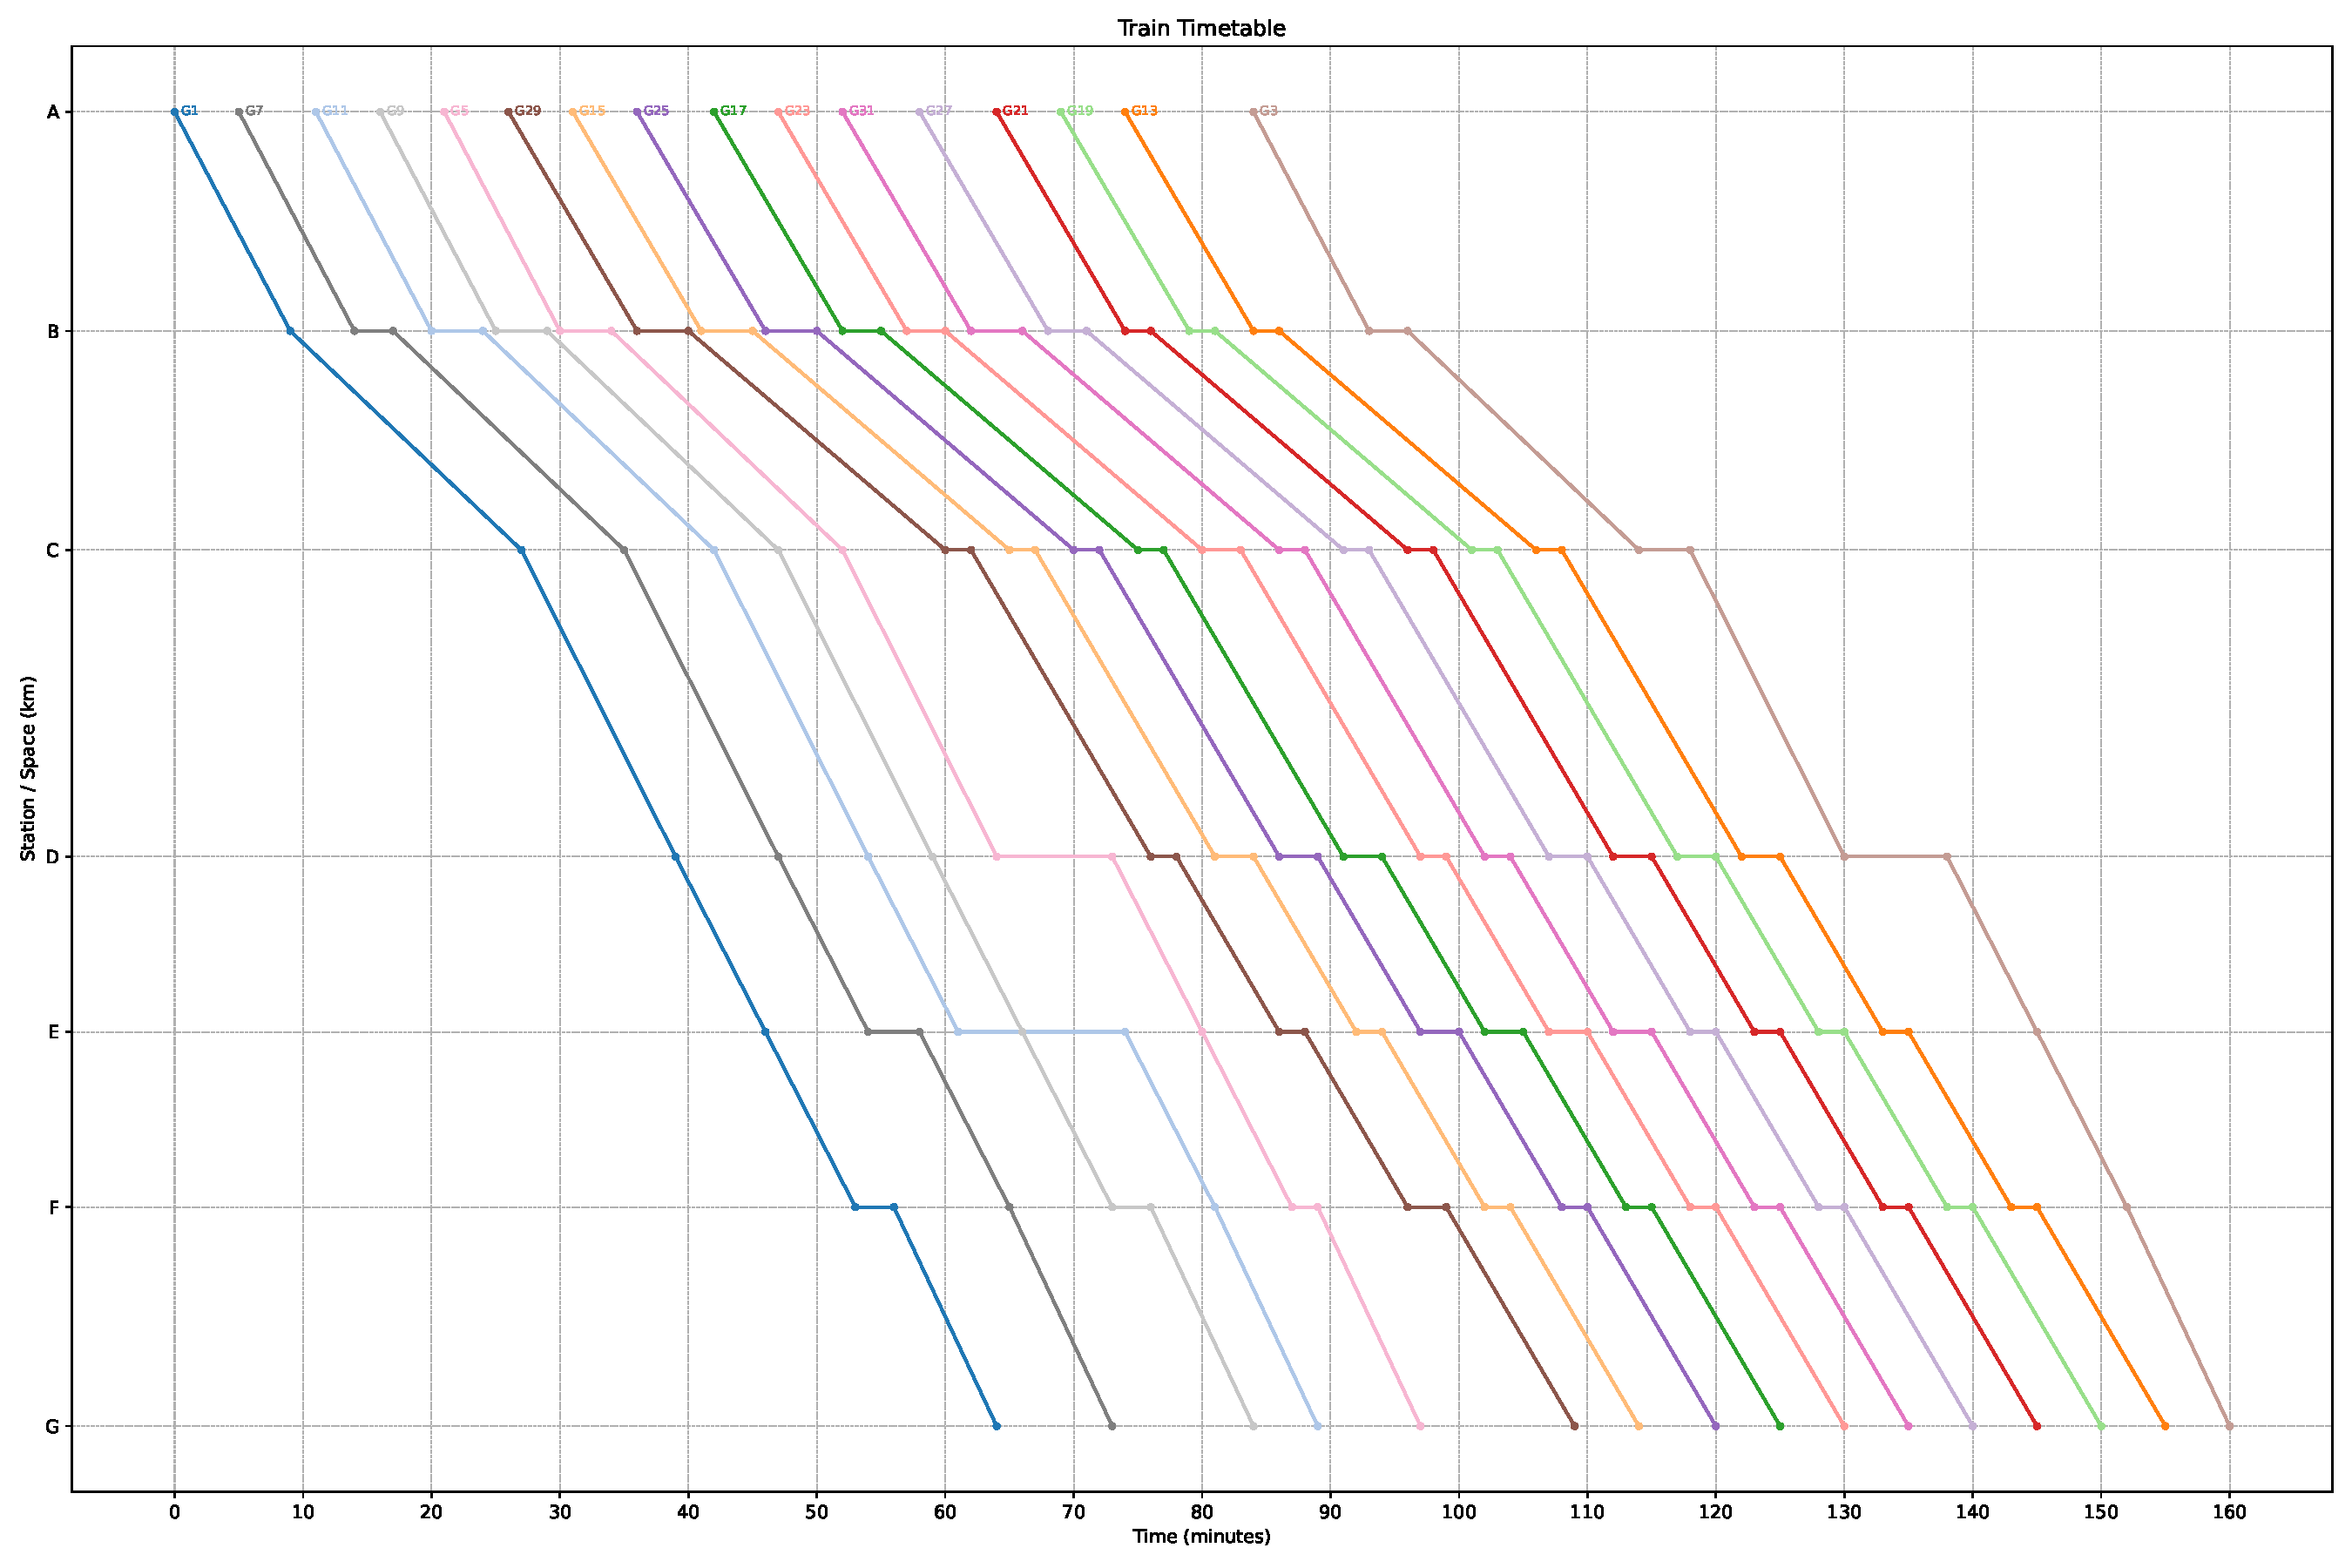
\includegraphics[width=0.7\textwidth]{fig/grb_feas}
    }
    \subfigure[gurobi\_solver\_min\_makespan]{
        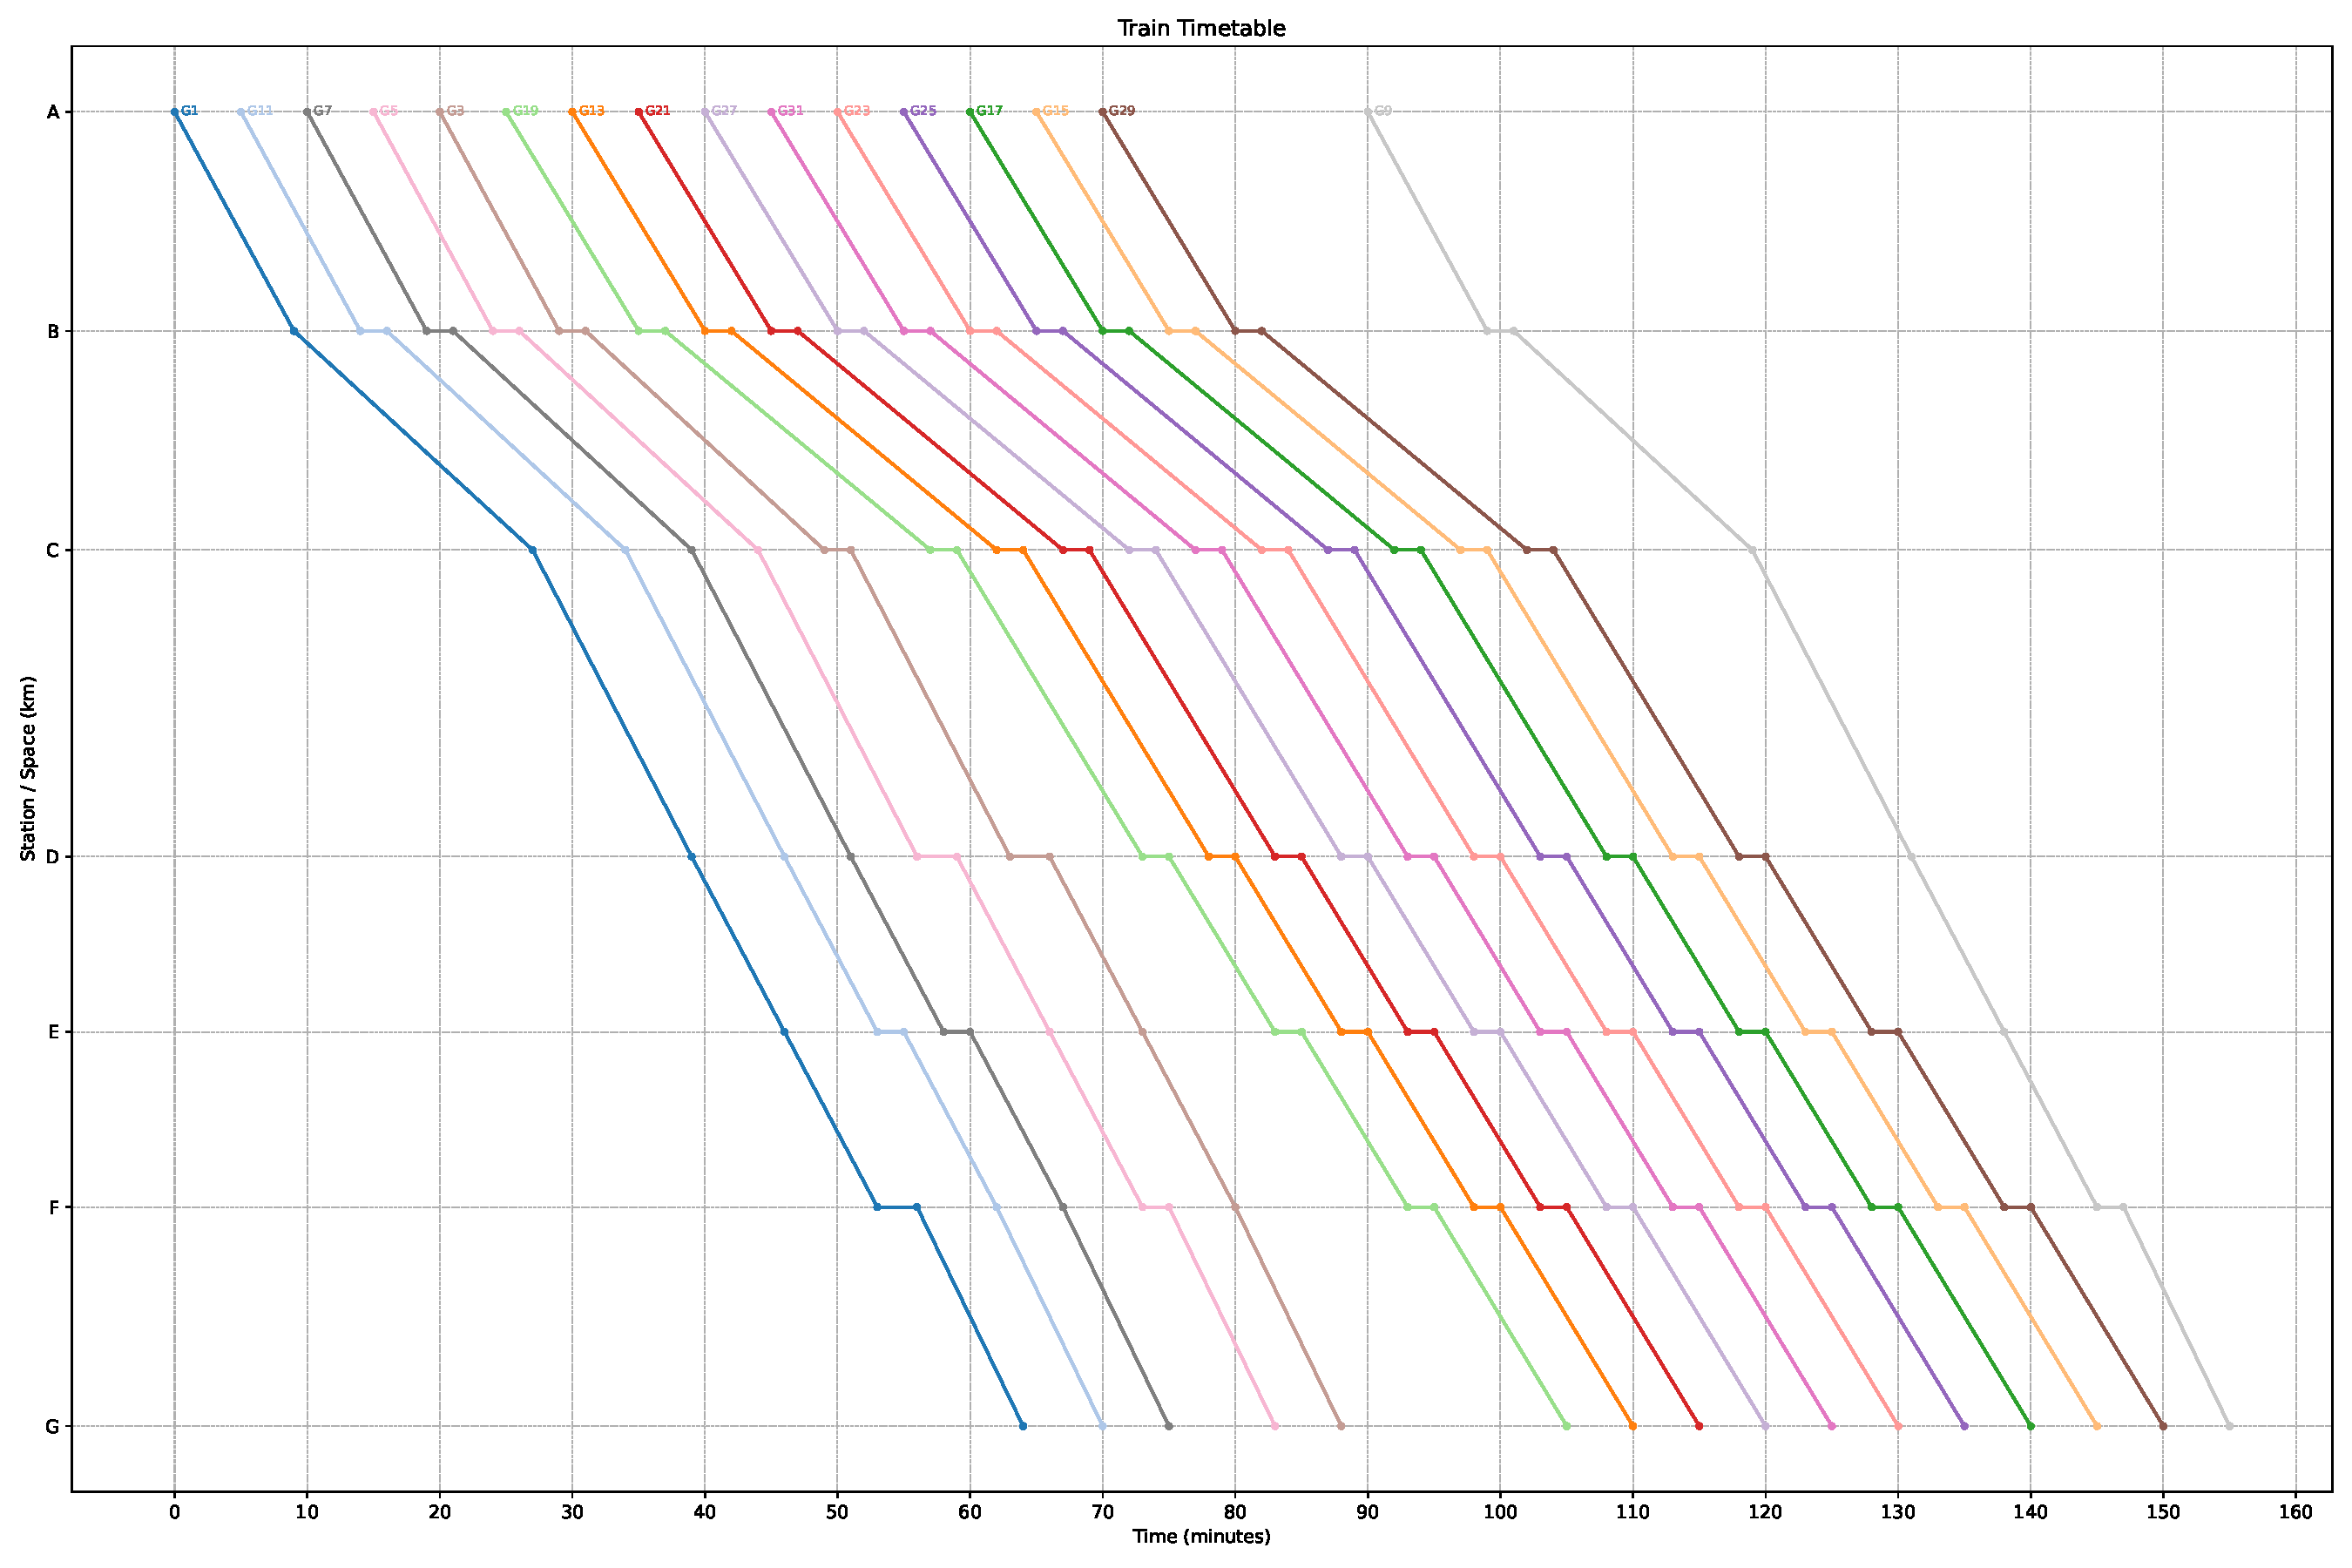
\includegraphics[width=0.7\textwidth]{fig/grb_min_makespan}
    }
    \subfigure[gurobi\_solver\_min\_arrive]{
        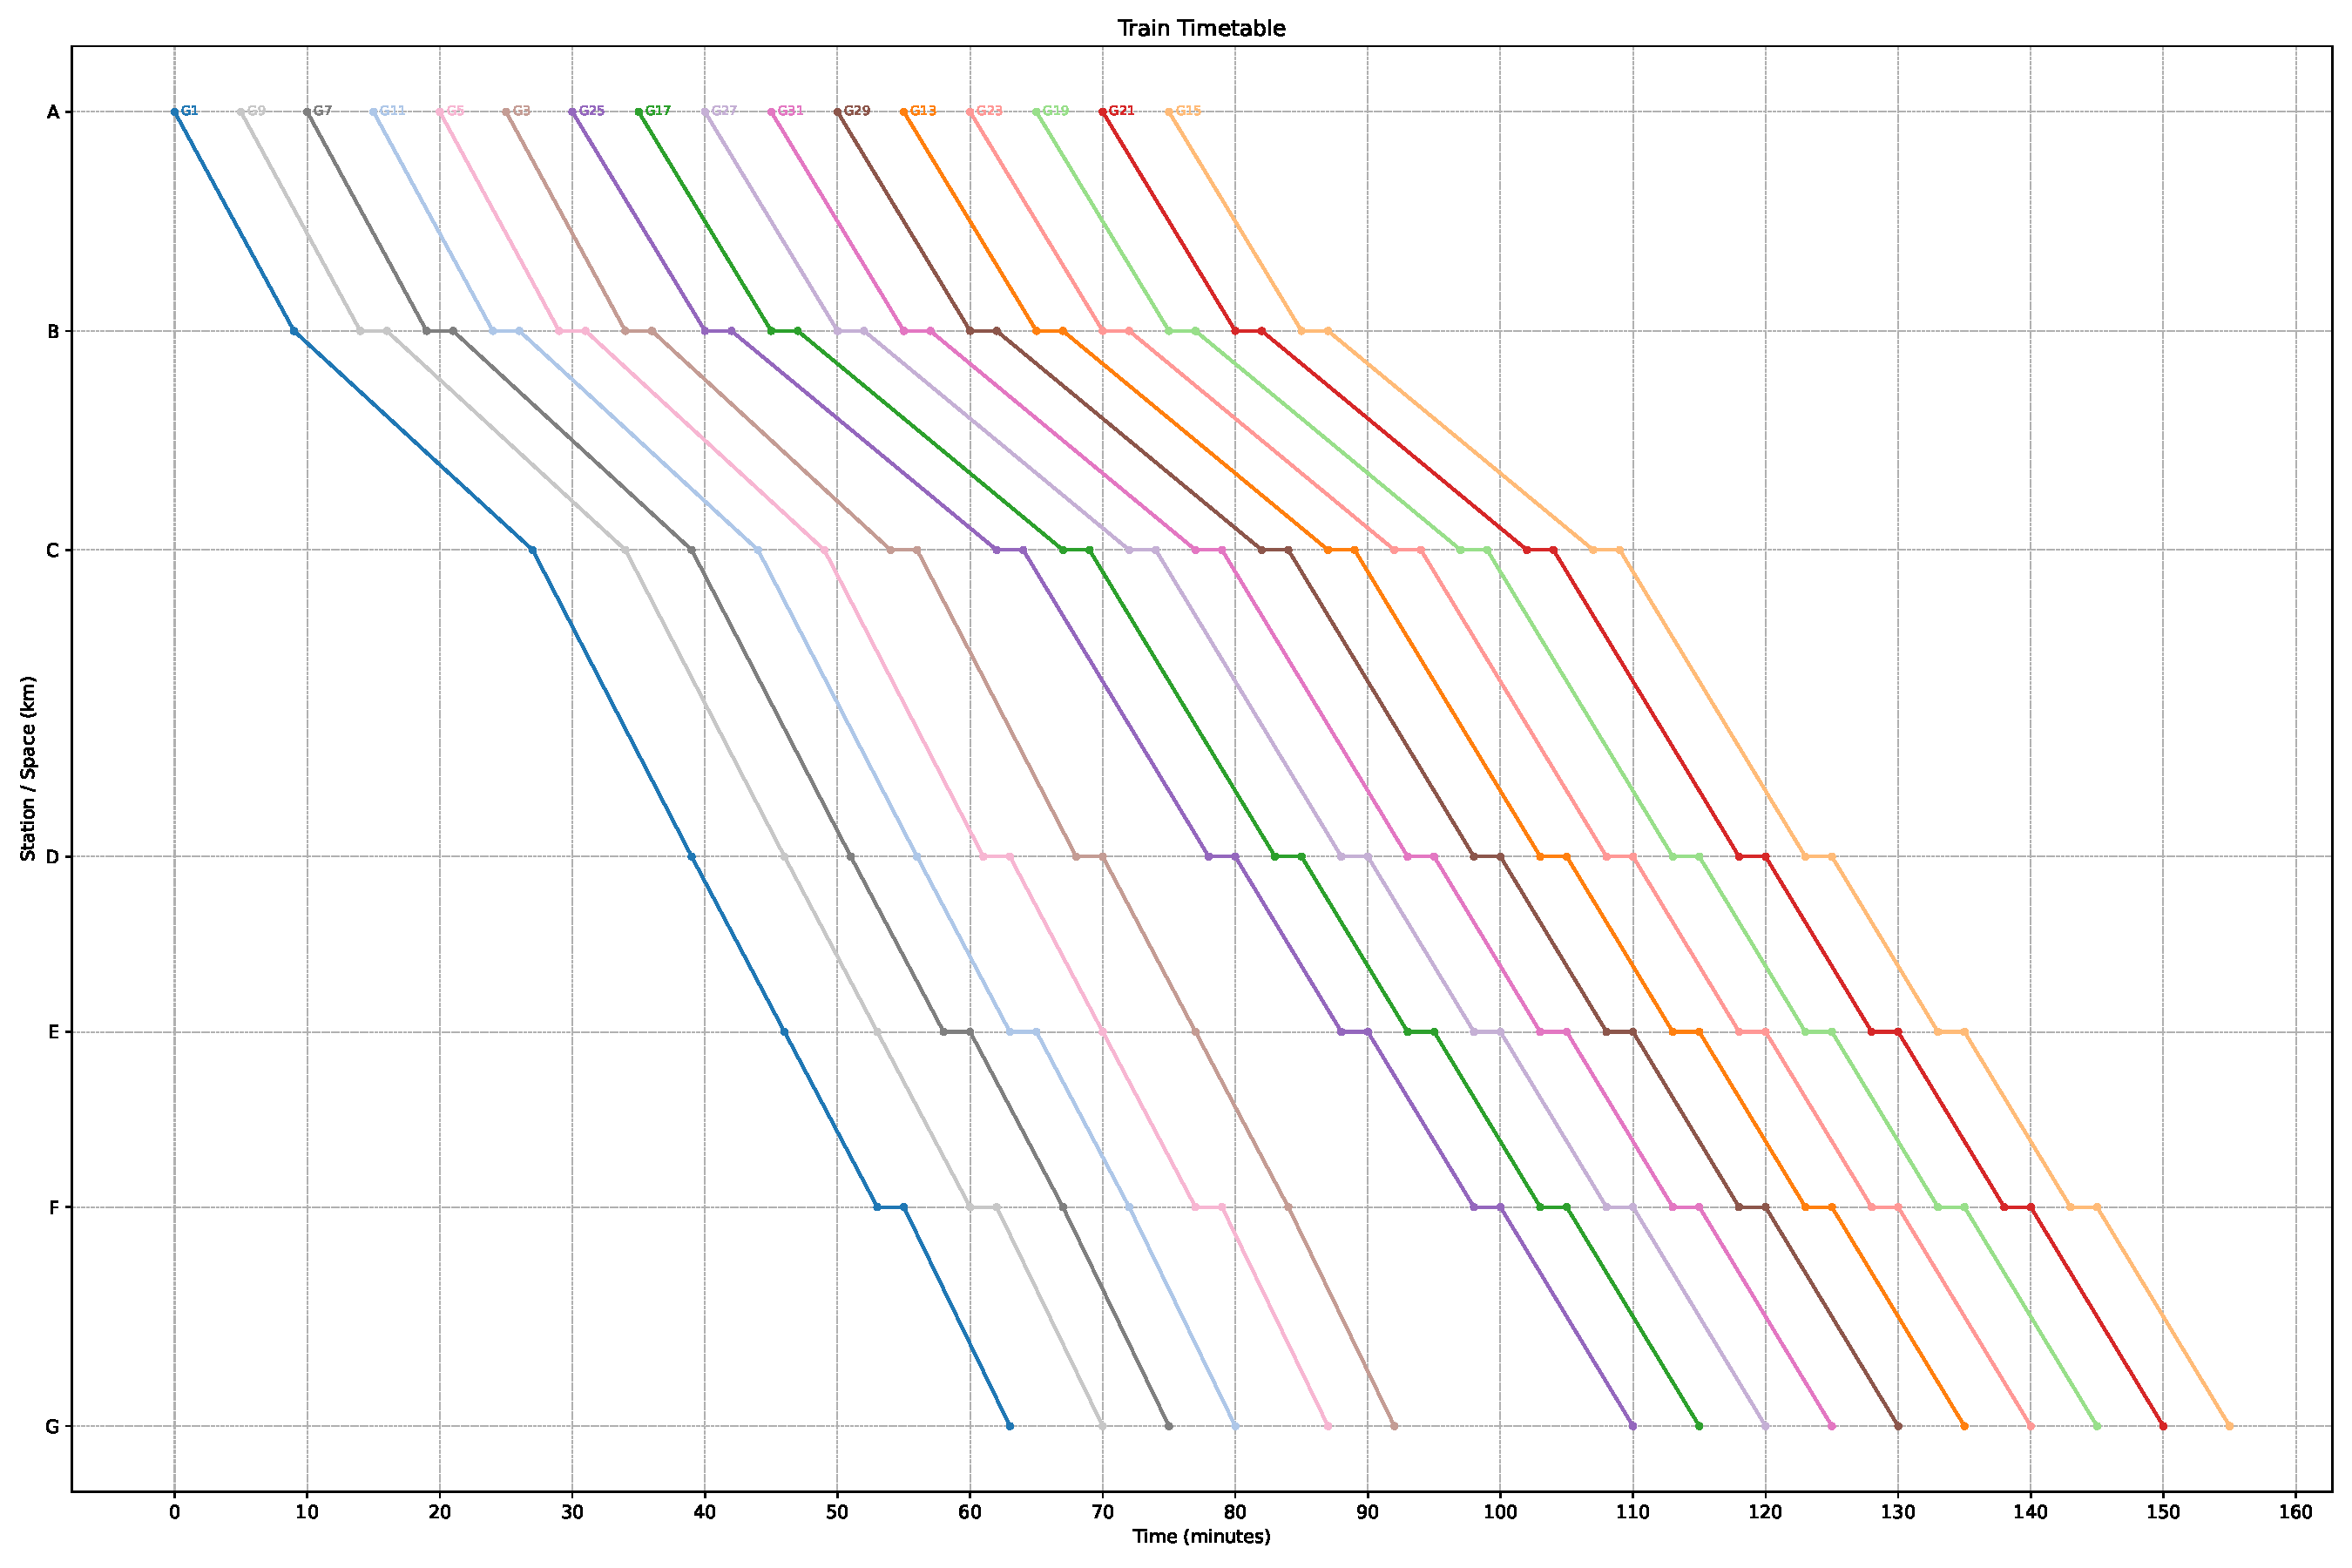
\includegraphics[width=0.7\textwidth]{fig/grb_min_arrive}
    }
    \caption{铁路时刻图(第一部分)}
    \label{fig:time_graph_1}
\end{figure}

\begin{figure}[htbp]
    \centering
    % 第二页放后 3 张图
    \subfigure[gurobi\_solver\_job\_shop\_feasibility]{
        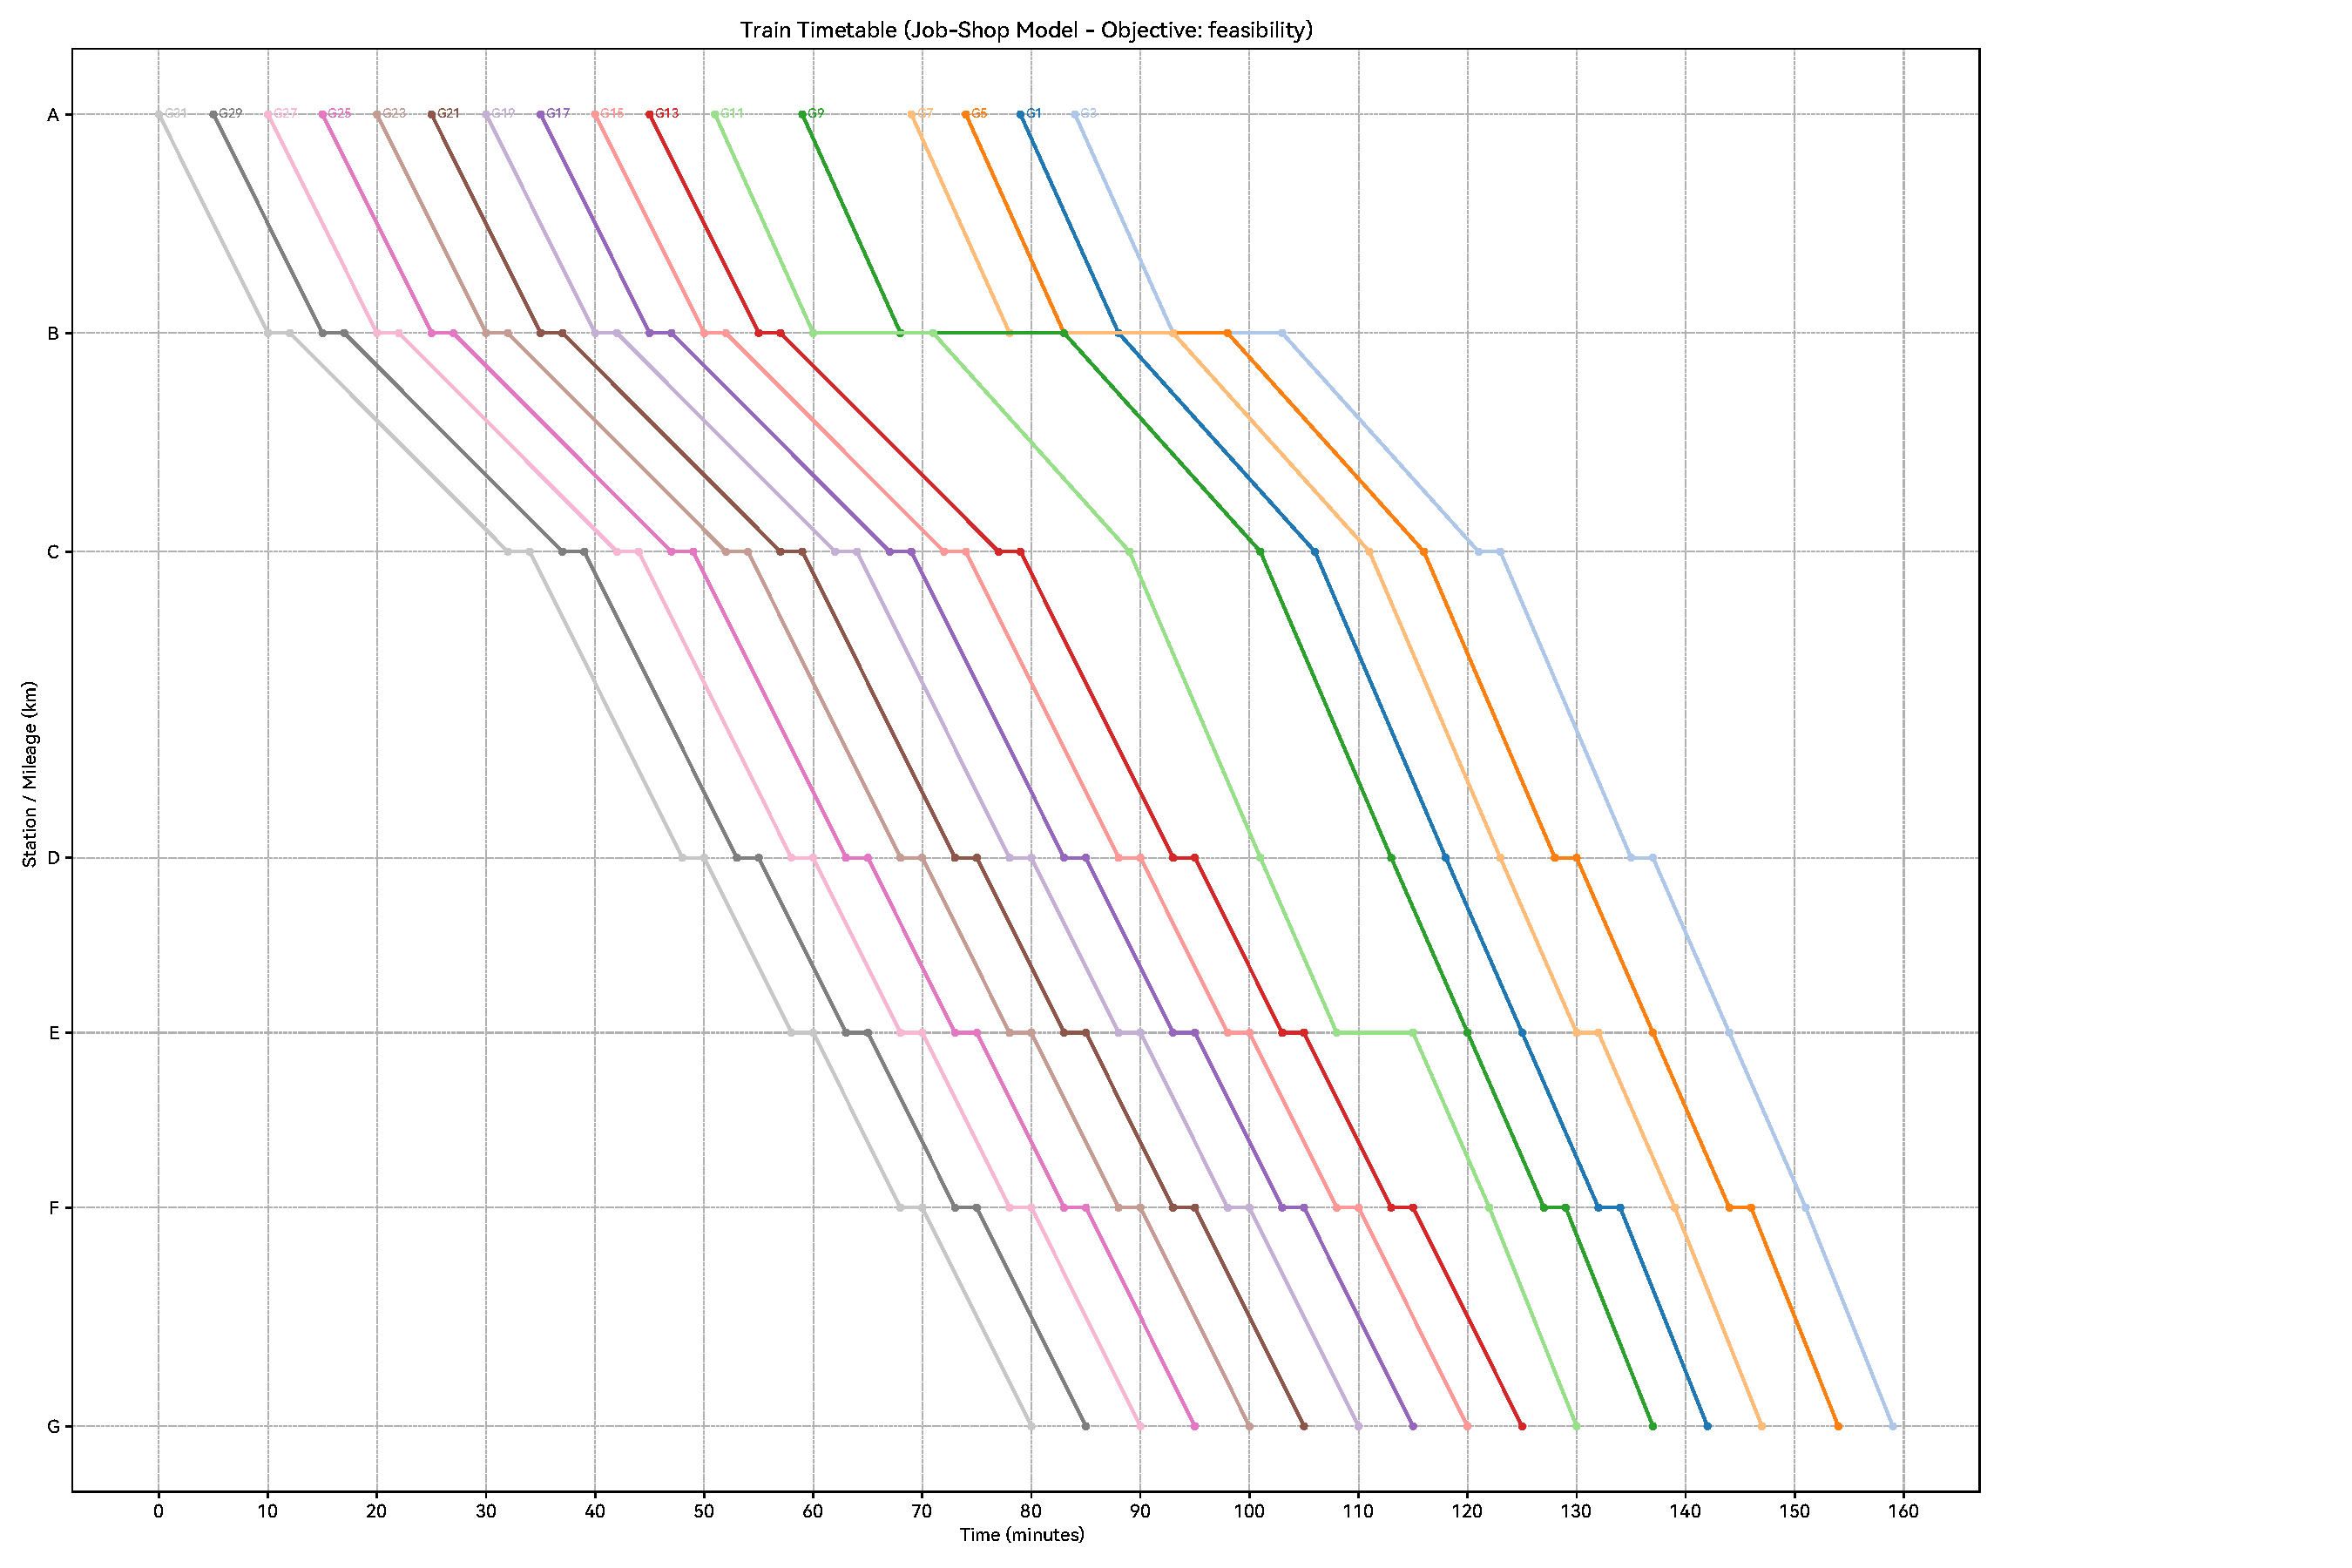
\includegraphics[width=0.7\textwidth]{fig/train_timetable_plot_jobshop_feasibility}
    }
    \subfigure[admm\_solver\_feasibility]{
        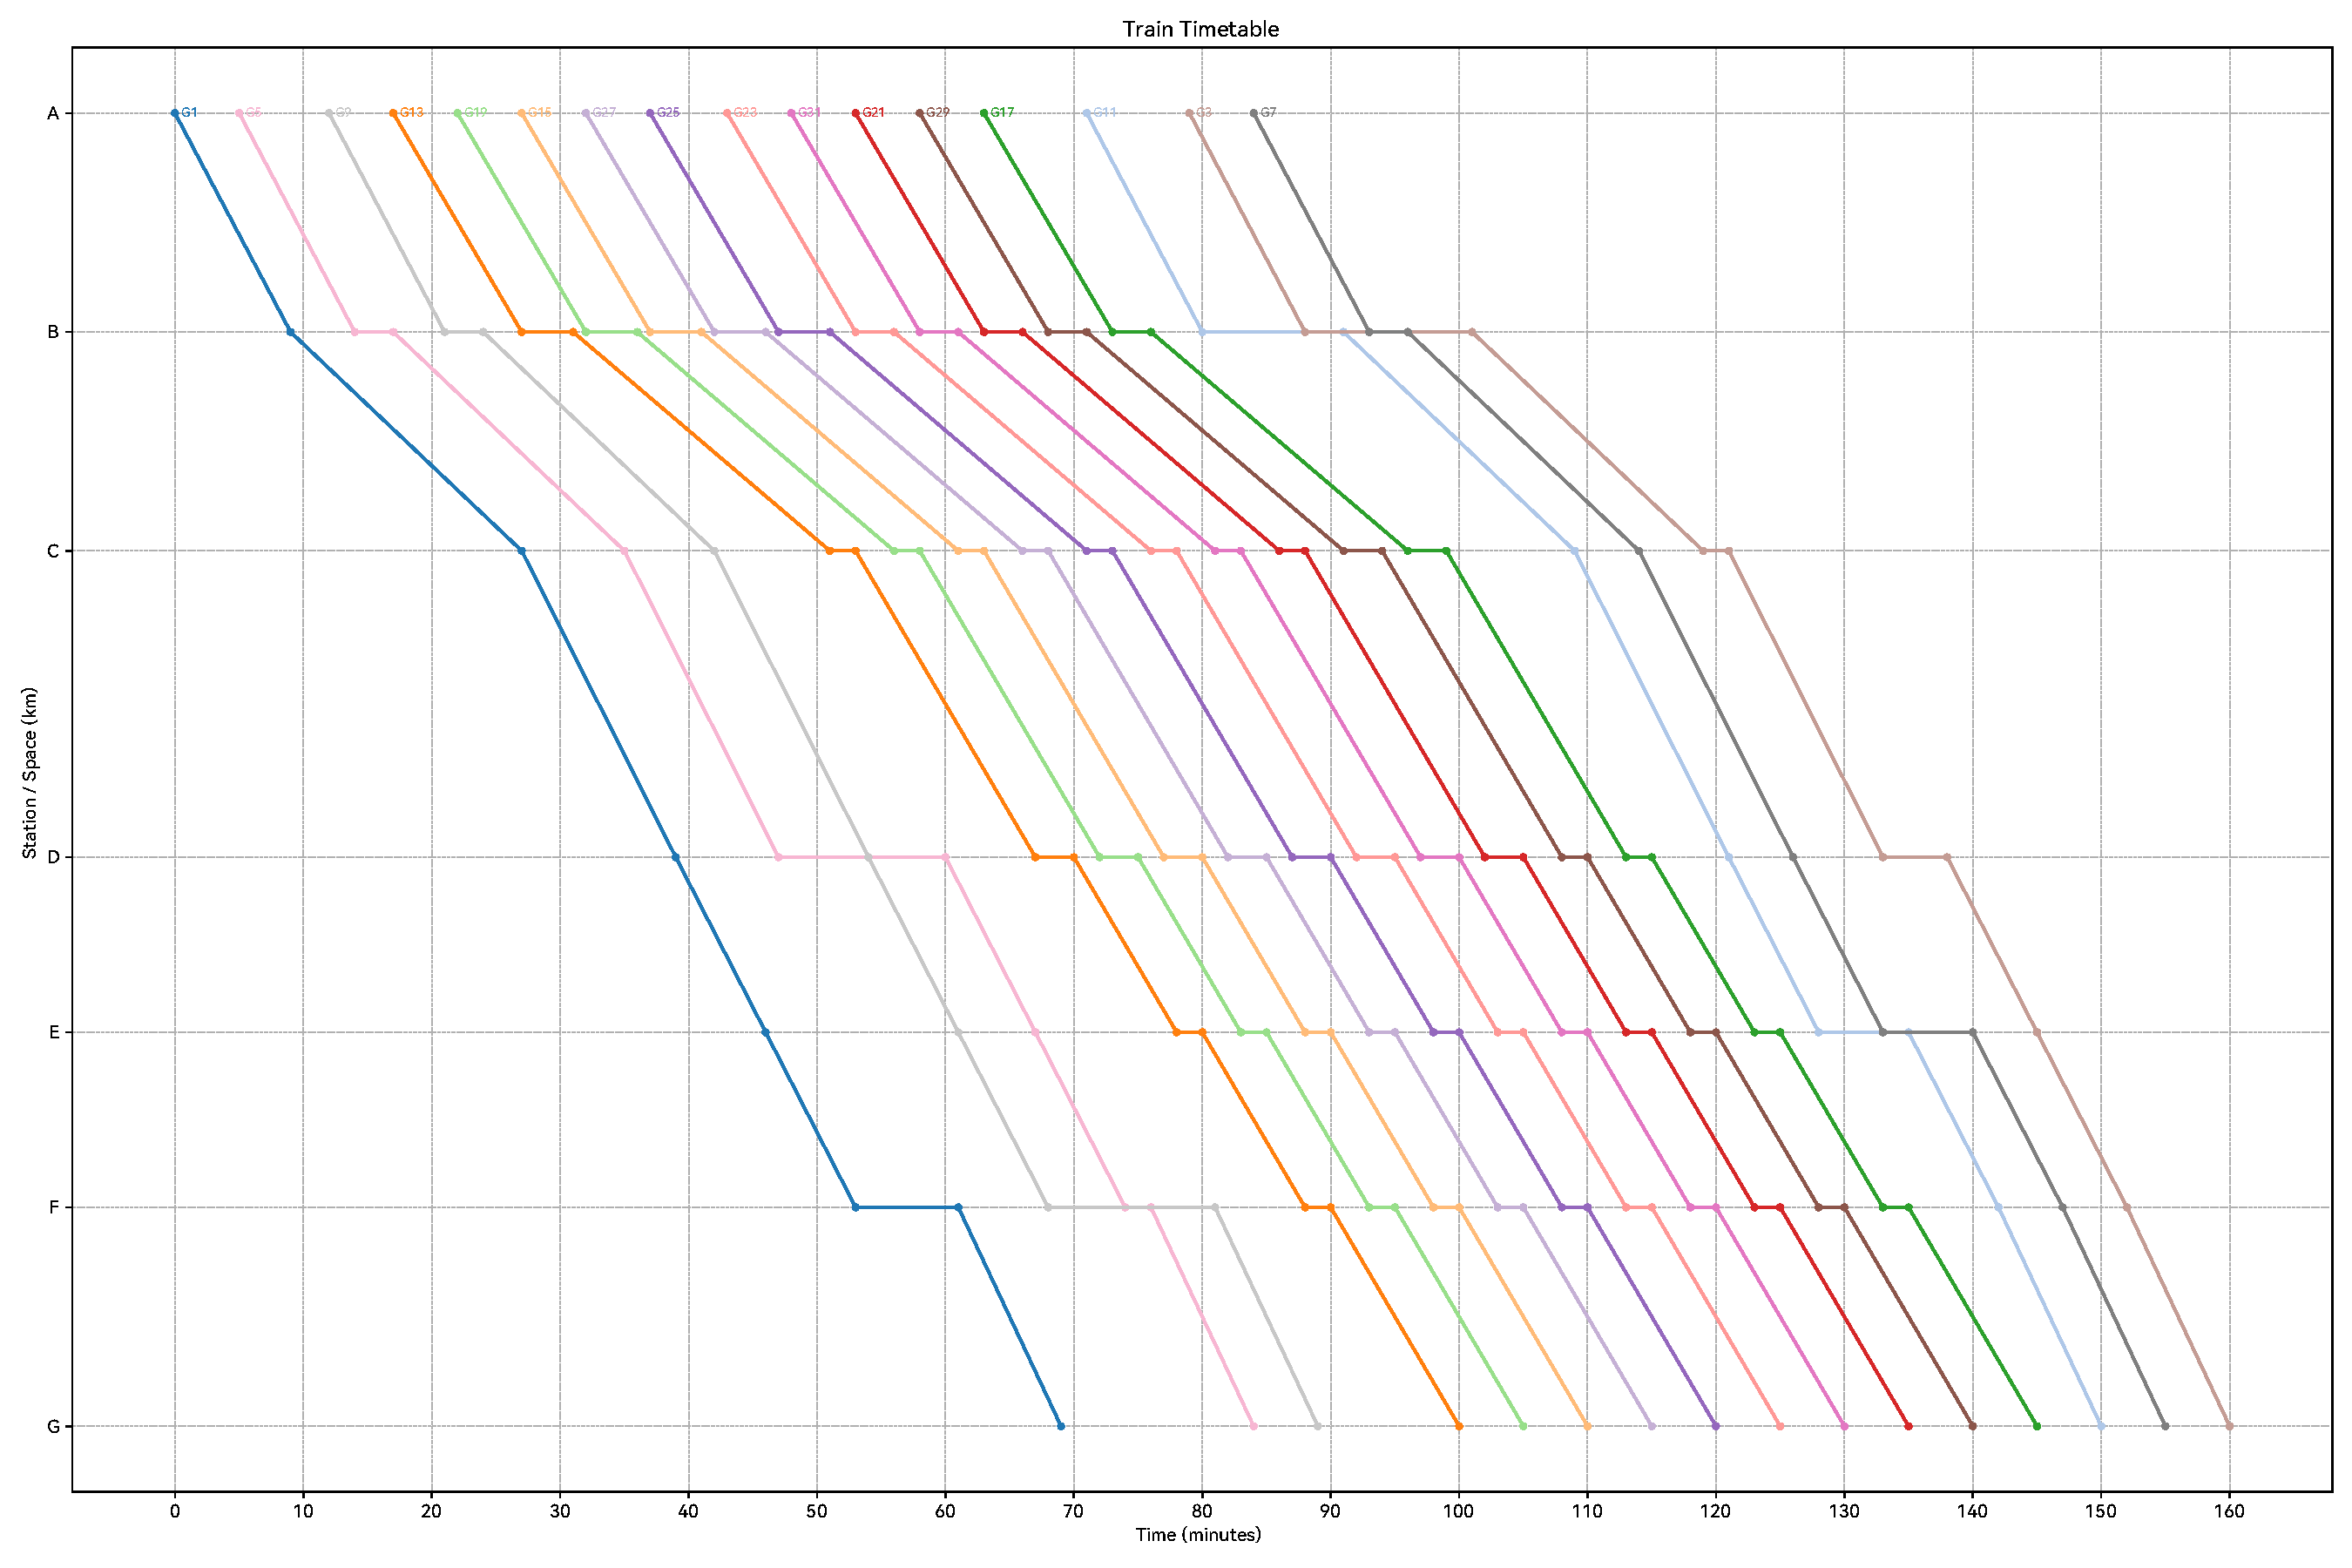
\includegraphics[width=0.7\textwidth]{fig/admm_timetable}
    }
    \subfigure[lagrange\_solver\_feasibility]{
        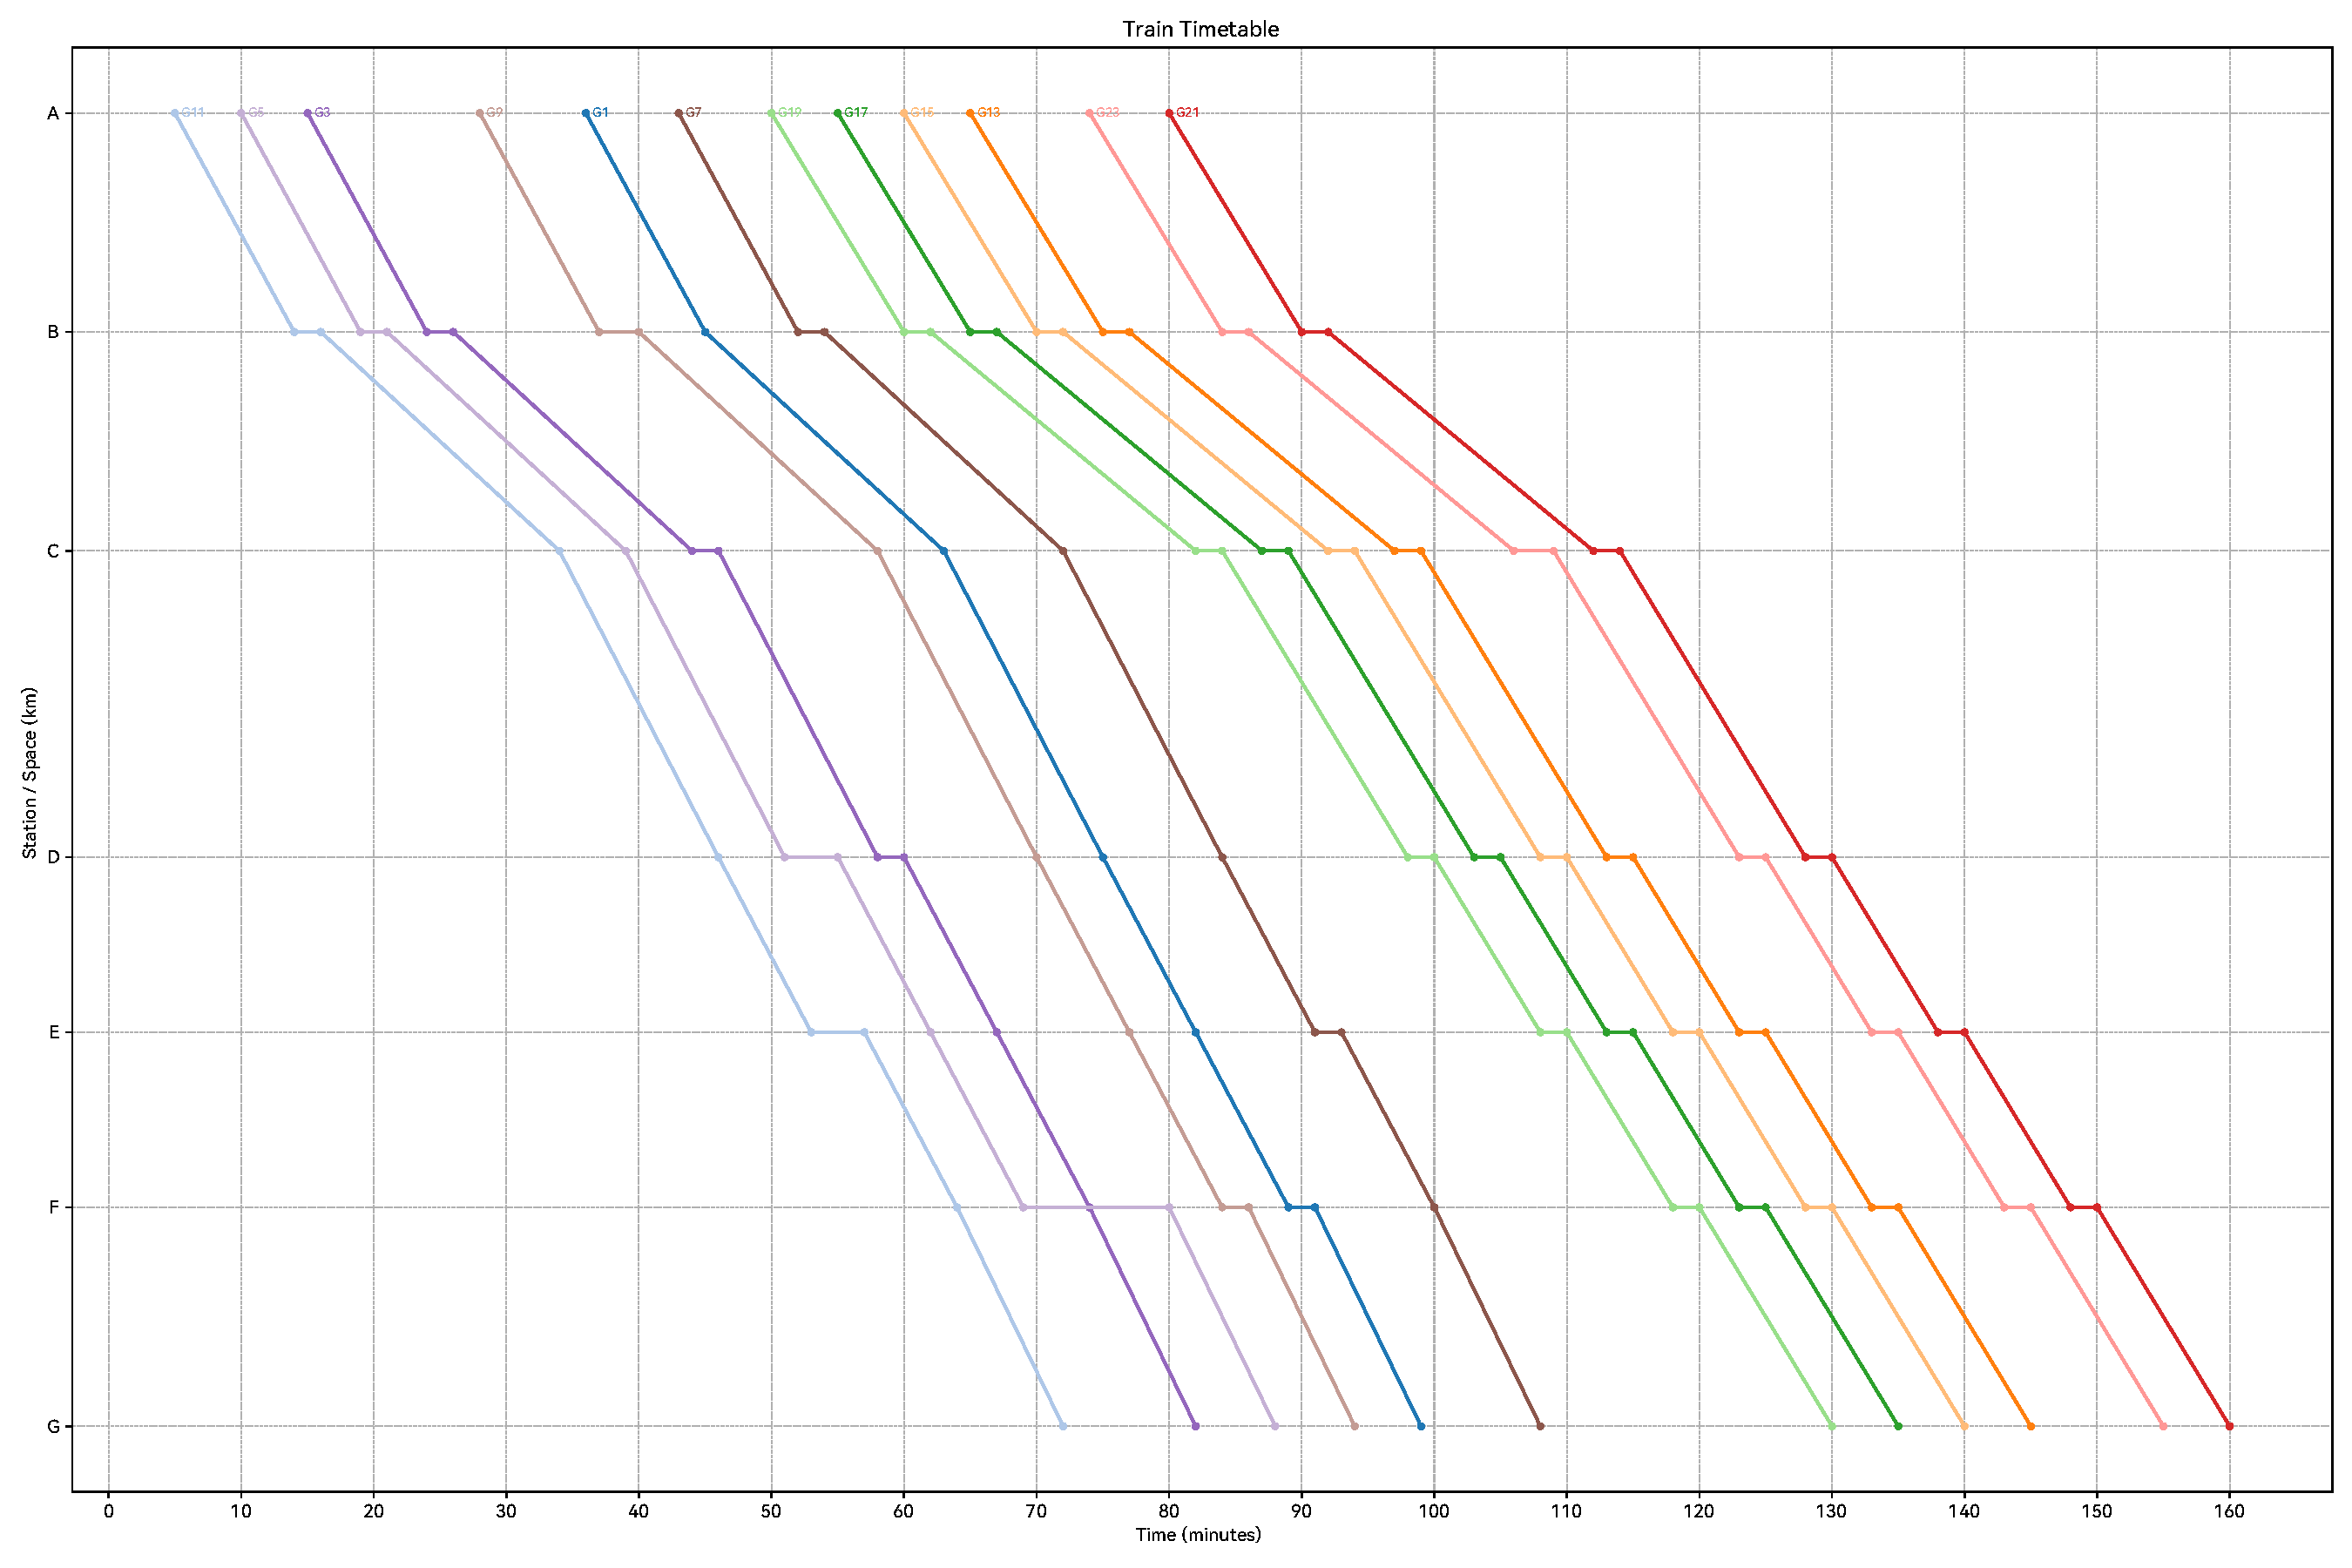
\includegraphics[width=0.7\textwidth]{fig/lagrange_timetable}
        \label{fig:time_graph_2_c}
    }
    \caption{铁路时刻图(第二部分)}
    \label{fig:time_graph_2}
\end{figure}

此外,我们还绘制了ADMM算法约束违反度随迭代次数变化的曲线,如图 \ref{fig:admm_infeasibility}
所示。可以看出,随着迭代次数的增加,约束违反度逐渐减小,最终趋于0,表明ADMM算法成功找到了可行解。

\begin{figure}
    \centering
    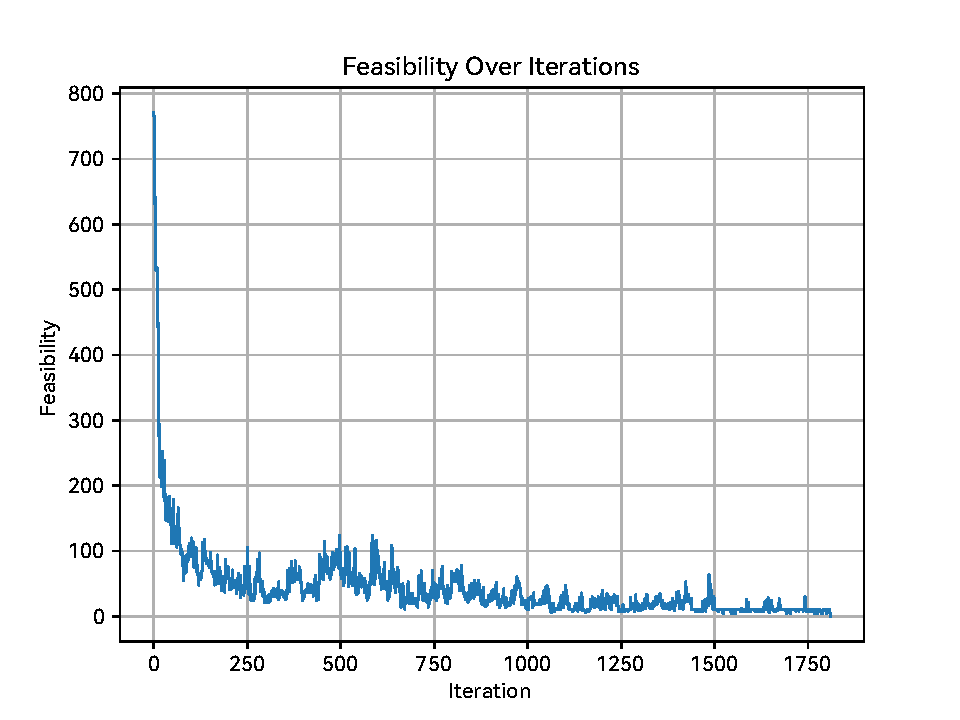
\includegraphics[width = 0.7\textwidth]{fig/admm_feas}
    \caption{ADMM算法约束违反度随迭代次数变化曲线}
    \label{fig:admm_infeasibility}
\end{figure}

\section{结果分析}

\subsection{模型与求解器性能对比}

\textbf{精确求解器 (Gurobi) 表现:}
实验结果表明,直接使用 Gurobi 求解器对整数规划模型进行求解,能够得到高质量的可行解或最优解。时空网络模型
(\texttt{gurobi\_solver}) 与 Job-Shop 模型 (\texttt{job\_shop\_solver})
相比,在求解可行性问题时,后者表现出显著的性能优势。Job-Shop 模型的运行时间仅为 1.40 秒,远快于时空网络模型的 129.95
秒。这主要归因于其模型规模的巨大差异:Job-Shop 模型仅用了 2352 个变量和 6111 个约束,而时空网络模型则需要多达
197678 个变量和 71299 个约束。这说明对于此类问题,一个更紧凑、更抽象的数学模型(如
Job-Shop)在求解效率上远优于直接建立的、规模庞大的时空网络模型。
在时空网络模型中,不同的优化目标对求解难度有显著影响。求解可行性问题
(\texttt{feasibility})的速度相对较快,而最小化最大完工时间 (\texttt{min\_makespan})和
最小化总到达时间
(\texttt{min\_arrive})则耗时较长(600秒以上),这是因为不仅仅满足可行性的目标函数会导致更复杂的搜索空间。从图
\ref{fig:time_graph_1}
中可以看出,不同的目标函数生成了视觉上存在差异的时刻表,例如 \texttt{min\_makespan}
和\texttt{min\_arrive}的时刻表在时间轴上更为紧凑,仅使用155分钟就完成了所有列车的调度,而
\texttt{feasibility} 的时刻表则相对松散,时间跨度更大。

\textbf{启发式/迭代算法表现:}
我们实现的拉格朗日松弛和 ADMM 算法作为启发式和迭代方法,展现了与精确求解不同的特性:
\begin{itemize}
    \item \textbf{ADMM 求解器 (\texttt{admm\_solver}):} ADMM 算法成功在
        270.39 秒内找到了一个可行解,证明了该方法在解决列车调度问题上的有效性。图
        \ref{fig:admm_infeasibility}
        清晰地展示了其收敛过程:随着迭代次数的增加,约束违反度单调下降并最终趋近于
        0,表明算法最终找到了满足所有约束的解。尽管其运行时间长于 Gurobi,但它提供了一种不依赖商业求解器的分布式优化思路。
    \item \textbf{拉格朗日松弛求解器 (\texttt{lagrange\_solver}):}
        我们实现的基于次梯度的拉格朗日松弛算法在限定的 1000 次迭代内未能为所有列车找到无冲突的路径,最终有 4
        辆列车未能安排,如图 \ref{fig:time_graph_2_c} 所示。其运行时间也最长,达到了 716.83
        秒。这表明,虽然拉格朗日松弛为求解大规模问题提供了理论框架,但其收敛速度和解的质量高度依赖于乘子更新策略、步长选择和启发式可行解构造等环节,需要精细的参数调整才能达到理想效果。
    \item \textbf{Gurobi 求解拉格朗日松弛问题 (\texttt{gurobi\_solver(LR)}):}
        作为对比,我们使用 Gurobi
        直接求解拉格朗日松弛后的问题。结果显示求解速度极快,但其解是不可行的,这符合预期,因为拉格朗日松弛问题的解仅为原问题提供了界限,而不保证满足被松弛的约束。
\end{itemize}

\subsection{结论}
综合来看,实验结果揭示了不同建模方法和求解算法在解决铁路列车时刻表问题时的性能权衡。 紧凑的 Job-Shop
模型在计算效率上远胜于庞大的时空网络模型,这对于处理更大规模的实际问题至关重要。
虽然商业求解器 Gurobi 能够为精确模型找到高质量解,但计算成本较高。而 ADMM
和拉格朗日松弛等迭代/启发式方法虽然在理论上更具扩展性,但在实践中需要复杂的参数调优,其性能和求解质量在本实验的规模下并未超越商业求解器。
本组成功给出了可行的列车运行图,其直观地反映了不同算法和优化目标下的调度结果,验证了算法的正确性,并展示了不同优化策略对最终时刻表形态的影响。

\section{LMM建模求解}

\subsection{Prompt设计}
近年来,大语言模型 (Large Language Models, LMMs)
的快速发展为解决复杂问题提供了新的思路和工具。在运筹优化领域,特别是在如列车运营时间表这样的复杂调度问题中,LMM展现出在问题理解、模型构建、代码生成乃至结果解释等多个环节辅助研究人员和工程师的潜力。
本组设计了自然语言prompt,用于询问大语言模型,得到铁路列车时刻表问题的建模,及相应求解代码,prompt的具体内容见\textbf{prompt.md}。在设计prompt的过程中,我们考虑了以下几个方面:
\begin{itemize}
    \item \textbf{问题描述的清晰性}: 采用先总后分的形式,确保问题描述准确且易于理解,避免歧义。
    \item \textbf{模型参数的定义}: 明确列车、车站、运行时间等关键参数的定义和范围。
    \item \textbf{约束条件的完整性}: 包括列车路径选择、节点占用、最小间隔等约束。
    \item \textbf{目标函数的多样性}: 提供多种优化目标,如最小化总到达时间、最大完工时间等。
    \item \textbf{代码生成的可执行性}: 指明需要使用 Python 语言及Gurobi求解器。
    \item \textbf{结果输出的格式}: 要求输出格式化的数学建模及可执行的代码,并提供必要的注释和文档说明。
\end{itemize}

\subsection{结果对比}
使用设计的prompt,我们分别向\textbf{Deepseek}的 V3-0324 和 R1-0528
两种模型发起询问,得到的回答见\textbf{v3.md}和\textbf{r1.md},经过测试,两种模型给出的代码均能正确运行并求解问题。以下是两种模型的回答对比:

\subsubsection{V3-0324 模型 (非推理模型)}
\begin{itemize}
    \item
        \textbf{优势:}高度贴合用户原始描述,其变量定义(如\texttt{x\_t,a}、\texttt{y\_s,$\tau$,t
        }、\texttt{z\_s,$\tau$ })和约束条件几乎是用户描述的直接翻译。
        展现了逐步修正能力,能在用户指出错误后定位问题并改进。
    \item
        \textbf{劣势:}初始生成的Gurobi代码存在错误,需要用户反馈后修正。数据结构与逻辑耦合较紧,例如流量守恒约束对活动元组内部索引的依赖,降低了对活动定义变化的灵活性和鲁棒性。
\end{itemize}

\subsubsection{R1 模型 (推理模型)}
\begin{itemize}
    \item \textbf{优势:}采取了更为抽象和通用的运筹学建模思路,引入核心数据结构
        \texttt{event\_mapping},清晰定义了网络节点、连接及活动对应的事件,增强了模型的结构化和可扩展性。
        决策变量 \texttt{z\_t,e} (列车\(t\)是否使用事件点\(e\))
        定义直接,便于构建“单一列车占用单个事件点”及“冲突集”的约束。
        约束表达清晰高效,如流量守恒、事件占用和冲突集约束均基于结构化数据。
        \texttt{event\_mapping}的设计使模型在很大程度上是数据驱动的,适应网络结构或活动细节的变化。
    \item \textbf{劣势:}\texttt{event\_mapping}
        结构相对复杂,用户需投入更多精力正确构建此映射表,初始数据准备门槛较高。模型需要消耗大量时间和计算资源进行推理,对于需要快速响应的应用场景不够高效。
\end{itemize}

综上,可以得出推理式模型在处理数学和编程问题时,展现出明显更强的能力。但两种模型均只能给出较为简单的模型和代码,无法直接满足对多辆列车进行复杂建模的需求

\end{document}